% !TEX root = ../../mat_738_alggeo.tex
\newpage
\section{Projective Varieties}
\subsection{Introduction}

Graded rings first.

\begin{dfn}[Graded Ring]
Let $R$ be a ring. A grading of $R$ is an expression of the additive group $(R,+)$ as an internal direct sum $R= \oplus_{i=1}^\infty R_i$ with the property that if $a \in R_d, b \in R_e$, then $ab \in R_{e+d}$, written $R_e \cdot R_d \subseteq R_{de}$. A graded ring is a ring together with a given grading. An element of $R_d$ is said to be homogeneous of degree $d$. 
\end{dfn}


\begin{ex}
Let $R= k[x_1,\ldots,x_n]$. $R_i= \{ f \in R \colon \text{all monomials of } f  \text{ having deg }i\} \cup \{0\}$, is homogenous of every degree. $\C[x,y]$, $x^2+4xy-17y^2$ is homogeneous of degree 2. $x^3-xy$ is not homogeneous. \xqed
\end{ex}


\begin{rem}
You can replace $\oplus_{i=0}^\infty R_i$ with $\oplus_{i \in M} R_i$, where $M$ is any monoid. We say the case of $\Z$ is $\Z$-grading. 
\end{rem}


Let $R$ be a graded ring. Each $f \in R$ has a unique expression $f= f_0 + \cdots + f_d$, where $f_i$ is homogeneous of degree $i$---simply the definition of a direct sum. 


















Definition and prop (homogeneous graded ideal)


\begin{prop}
Let $R$ be a graded ring and $I \subseteq R$ be an ideal. The following are equivalent:
\begin{enumerate}[(i)]
\item $I$ can be generated by homogeneous elements
\item $I= \oplus_{i=0}^\infty (I \cap R_i)$ as a group
\item given $f \in R$, write $f= f_0 + \cdots + f_d$, where $f_i$ is homogeneous of degree $i$. Then $f \in I$ if and only if all $f_i \in I$. 
\end{enumerate}
\end{prop}

\pf (b) if and only if (c) definition of direct sum. In (c), note that all $f_i \in I$ certainly $f \in I$. The only things to check is $f \in I$, then $f_i \in I$. (c) to (a): write every $f \in I$ as $f= f_0 + \cdots + f_d$, where $f_i$ is homogeneous of degree $i$. Certainly, $I$ is generated by all the $f_i$ that appear as $f$ varies over all $f \in I$. (a) to (c): Say $I$ is generated by $\{f_\alpha\}$, $\alpha \in A$, where $f_\alpha$ is homogenous of degree $d_\alpha$. Choose $F \in I$, then $F= \sum_{i=1}^n a_i f_{\alpha_i}$. Write $F= F_0 + \cdots + F_d$, where $F_j$ is homogeneous of degree $j$. What is $F_j$ in terms of the expression?
	\[
	F_j= \sum_{i=1}^n ((\text{deg }j - \text{deg}(f_{\alpha_i})) \text{ piece of }a_i) f_{\alpha_i \in I}. 
	\] \qed \\


\begin{prop}
Let $R$ be a graded ring.
\begin{enumerate}[(i)]
\item if $I, J$ are homogeneous ideals, then so are $I+J$, $IJ$, $I \cap J$, and $\sqrt{J}$
\item let $I$ be a homogeneous ideal. Then $I$ is prime if and only if for any two homogeneous elements $f,g \in R$, if $fg \in I$ then either $f \in I$ or $g \in I$. 
\item if $f,g \in R$, and integral domain, with $f,g$ nonzero, then $fg$ is homogeneous if and only if $f,g$ are homogeneous. 
\end{enumerate}
\end{prop}


\pf 

$f= f_0 + \cdots + f_d$, $g= g_0 + \cdots+ g_e$
$fg= (f_dg_e) + (f_{d-1}g_e+ f_dg_{e-1}) + \cdots$
If all $f_i \in I$, then $F \in I$ and we are done.
If all $g_i \in I$, then $g \in I$ and we are done.
So assume that $f_i \notin I$ and some $g_j \notin I$.
Let $s$ be the largest number such that $f_s \notin I$ and let $t$ be the largest number such that $g_t \notin I$. We examine the degree $s+t$ piece of $fg$ as $fg \in I$ and $I$ is homogeneous, it is in $I$. It will have the form $f_sg_t+$ terms of the form $f_ig_j$ with either $i>s$ or $j>t$. All of these extra terms are in $I$, the whole sum is in the ideal. Thus, $f_sg_t \in I$ then either $f_s \in I$ or $g_t \in I$, a contradiction. \qed \\


For a homogeneous ideal $I$ of $R$, we often denote $I \cap R_i$ by $I_i$. It then follows that 
	\[
	R/I \cong \dfrac{\oplus R_i}{\oplus I_i} \cong \oplus_{i=0}^\infty R_i/I_i.
	\]
Thus, $R/I$ is naturally a graded ring with $(R/I)_i = R_i/I_i$. Now suppose $R$ is a noetherian graded ring and $I \subset R$ is a homogeneous ideal. We know $I$ can be generated by homogeneous ideal because it is homogeneous. Because $R$ is noetherian, $I$ can be generated by finitely many elements. Can it be generated by finitely many homogeneous elements? Indeed, this is the case. If you set up the proof of the ACC then every ideal is f.g., you can prove ACC then every set of generators for an ideal has a finite subset that generates. 



Now for projective space, you may have heard `parallel lines meet at infinity'. 

% Give image of parallel railroad tracks meeting at infinity. 

The basic idea is to `compactify' $\A^n$ by adding `points at infinity'. This is similar to the way $\R^1$ is compactified to $S^1$ or $\R^2$ to $S^2$. This is not at all apparent from the initial definition of porjective space, but will eventually become clear. 


Consider $\A^{n+1}$ with coordinates $x_0,x_1,\ldots,x_n$. On $\A^{n+1} \setminus \{(0,\ldots,0)\}$, we define the following equivalence relation: $(a_0,\ldots,a_n) \sim (b_0,\ldots,b_n)$ if and only if there exists $\lambda \in k^\times$ such that $(a_0,\ldots,a_n)= (\lambda b_0,\ldots,\lambda b_n)$. The equivalence class of $(a_0,\ldots,a_n)$ is the one-dimensional subspace of $\A^{n_1}$ spanned by $(a_0,\ldots,a_n)$---minus the origin, which is the line through the origin and $(a_0,\ldots,a_n)$ minus the origin. 


\begin{dfn}
Projective $n$-space over $k$, denoted $\bP_k^n$ or $\bP^n(k)$ or $\bP= \A_k^{n+1} \setminus \{(0,\ldots,0)\}/\sim$. A point $P \in \bP$ is an equivalence class of some point $(a_0,\ldots,a_n) \in \A^{n+1} \setminus \{(0,\ldots,0)\}$ and is denoted $[a_0,\ldots,a_n]$. The $a_i$ are called the homogeneous coordinates of the point $P$. They are well defined up to a nonzero constant multiple. $\bP$ is also the set of lines through the origin in $k^{n+1}$, the set of one-dimensional subspaces of $k^{n+1}$. 
\end{dfn}



Denote the polynomial ring $k[x_0,\ldots,x_n]$ by $S$. For $f \in S$ and $O \in \bP^n$, $f(P)$ is not well defined because the coordinates of $P$ are not well defined. But suppose $f \in S$ is homogeneous: $f(\lambda a_0,\ldots, \lambda a_n) = \lambda^{\deg f} f(a_0,\ldots,a_n)$. $f(P)$ still not well defined since $\lambda \in k^\times$, whether $f(P)=0$ is well defined. So we define for a homogeneous $f \in S$, we define the zeros of $f$, denoted $Z(f)$ by $Z(f)= \{ P \in \bP^n \colon f(P)= 0\}.$ For a set of homogeneous elements $T \subseteq S$, we define the zeros of $T$, denoted $Z(T)$ by $Z(T)= \cap_{f \in I} Z(f)= \{P \in \bP^n \colon f(P)=0 \text{ for all }f \in T\}$. A set $Y \subseteq \bP^n$ is called algebraic if and only if $Y= Z(T)$ for some subset $T \subseteq S$ of homogeneous elements. If $I \subseteq S$ is a homogeneous ideal, we define $Z(I)= \{ P \in \bP^n \colon f(P)=0 \text{ for all homogeneous } f \in I\}= \cap_{f \in I, f homog} Z(f)$.


\begin{prop}
Let $T \subseteq S$ be a set of homogeneous elements, and let $I \subseteq S$ be the homogenous ideal generated by $T$. Then $Z(T)= Z(I)$. Thus, every algebraic set in $\bP^n$ is of the form $Z(I)$ for a homogeneous ideal and $Z(\{(f_1,\ldots,f_r)\})$ for finitely many homogeneous $f_i$, $Z(f_1,\ldots,f_r)$. 
\end{prop}


The algebraic subsets of $\bP^n$ satisfy the properties needed to be the closed subsets of a topology on $\bP^n$, it is the Zariski topology. 


\begin{dfn}
A projective algebraic variety (or simply projective variety) is an irreducible algebraic set in $\bP^n$, with the induced topology. An open subset of a projective variety is a quasi-projective variety. The dimension of a variety or quasi-projective variety is its dimension as a topological space. If $Y$ is any subset of $\bP^n$, we define the homogeneous ideal of $Y$ in $S$, denoted $I(Y)$, generated by $\{ f \in S \colon f \text{ homogeneous and } f(P)=0 \text{ for all }P \in Y\}$. If $Y$ is an algebraic set, we define the set of homogeneous coordinate ring of $Y$ to be $S(Y):= S/I(Y)$.
\end{dfn}


Note that $I(Y)$ is a homogeneous ideal so $S(Y)$ is a graded ring. These are similar to old algebraic sets with one funny difference. $S$ is clearly a homogeneous ideal of $S$. $Z(S)= \emptyset$, $S= k[x_0,\ldots,x_n]$ $(x_0,\ldots,x_n)$ is also clearly a homogeneous ideal of $S$. It is often called $S_+$ because it contains all homogeneous elements of positive degree $Z(S_+)= \emptyset$. This is the only thing which goes awry. $S_+$ is sometimes called the irrelevant maximal ideal since it removed from the correspondence we saw in the affine case. 


We now work on showing $\bP^n$ is $\A^{n+1}$ with points added at $\infty$. In $\bP^n$, consider closed sets of the form $Z(f)$ with $f$ a nonconstant polynomial These are called hypersurfaces. When $f$ is linear, it is called a hyperplane. Of particular interest is when $f= x_i$ for some $i$. Set $H_i= Z(x_i)= \{[a_0,\ldots,a_n] \;|\; a_i=0 \}$ and $U_i= \bP^n \setminus H_i$, $i=0,\ldots,n$, $U_i$ open. The $U_i$ are an open cover of $\bP^n$
	\[
	(\cup_i^n U_i)^C= \cap_0^n U_i^C= \cap_0^n H_i= \{[a_0,\ldots,a_N] \colon a_i= 0 \text{ all }i\}= \emptyset. 
	\]










































%%%%

$P= [a_0,\ldots,a_n] \in U_i$ if and only if $P= [a_0/a_i,\ldots,a_{i-1}/a_i,1,a_{i+1}/a_i,\ldots,a_n/a_i]$. Each point in $U_i$ has a unique set of homogeneous coordinates such that the $i$th coordinate is 1. Define a map $\phi_i: \A^n \to U_u$  by $\phi_i(a_1,\ldots,a_n)= [a_1,a_2,\ldots,1,\ldots,a_n]$. Moreover, this is clearly a bijection. 



\begin{prop}
The map $\phi_i$ is a homeomorphism of $U_i$ with its induced topology to $\A^n$ with its Zariski topology. 
\end{prop}

The proof is based on homogenization and dehomogenization of polynomials. To make notation simpler, we assume $i=0$. Let $S= k[x_0,\ldots,x_n]$, $A= k[x_1,\ldots,x_n]$, and $S^h$ denote the homogeneous elements of $S$. There is a ring homomorphism $\alpha: S \to A$, defined as evaluation at $x_0= 1$: $\alpha(f(x_0,\ldots,x_n))= f(1,x_1,\ldots,x_n)$. Since $\alpha$ is a ring homomorphism
	\[
	\begin{split}
	\alpha(f+g)&= \alpha(f)+\alpha(g) \\
	\alpha(fg)&= \alpha(f)\alpha(g),
	\end{split}
	\]
called dehomogenization because even if $f$ is homogeneous, $\alpha(f)$ may not be: $\alpha(x_0^2+x_0x_1)= 1+x_1$. 


Homogenization: $\beta: A \to S^h$: $\beta(f(x_1,\ldots,x_n))= x_0^{\deg f} f(x_1/x_0,\ldots,x_n/x_0)$, $\beta(f)$ is homogeneous of degree $\deg f$. Look at a monomial of $f$: $x_1^{i_1} x_2^{i_2} \cdots x_n^{i_n}$, $i_1+\cdots+i_n \leq \deg f$.
	\[
	x_0^{\deg f} (x_1/x_0)^{i_1} \cdots (x_n/x_0)^{i_n}= x_0^{\deg f - (i_1+\cdots+i_n)} x_1^{i_1} \cdots x_n^{i_n}
	\]
has degree $\deg f$.


$\beta(fg)= \beta(f) \beta(g)$.
$\beta(fg)= x_0^{\deg f + \deg g} f(x_1/x_0,\ldots,x_n/x_0) g(x_1/x_0,\ldots,x_n/x_0)= x_0^{\deg f} f(x_1/x_0,\ldots,x_n/x_0) x_0^{\deg g} g(x_1/x_0,\ldots,x_n/x_0)= \beta(f) \beta(g)$. $\beta(f+g)$ might not equal $\beta(f) + \beta(g)$. 

If $\deg f \neq \deg g$, $\beta(f) + \beta(g)$ will not even be homogeneous. 

If $\deg f= \deg g= \deg(f+g)$, then $\beta(f+g)= \beta(f) + \beta(g)$. 
	\[
	\alpha(\beta(f))= \alpha(x_0^{\deg f} f(x_1/x_0,\ldots,x_n/x_0)= 1^{\deg f} f(x_1/x_0,\ldots,x_n/x_0)= f
	\]
$\beta(\alpha(f))= \beta(\alpha(x_0^l f))$. Assume you have a homogeneous $F$ that is not divisible by $x_0$.
	\[
	F= \sum a_{i_0 \cdots i_n} x_0^{i_0} \cdots x_n^{i_n}
	\]
where $i_0 + \cdots + i_n= d$. 


$\alpha(F)= \sum a_{i_0 \cdots i_n} x_1^{i_0} \cdots x_n^{i_n}$ and in at least one case $i_1+ \cdots + i_n = d$. 

$\beta(\alpha(F))= x_0^d a_{i_0 \cdots i_n} ((x_1/x_0)^{i_0} \cdots (x_n/x_0)^{i_n}= F$. Consider a point $(a_1,\ldots,a_n) \in \A^n$. $\phi_0(a_1,\ldots,a_n)= [1,a_1,\ldots,a_n] \in U_0 \subseteq \P^n$. 

$f \in k[x_1,\ldots,x_n]$
$F \in k[x_0,\ldots,x_n]$ $F$ homogeneous
$f(a_1,\ldots,a_n)= 1^{\deg f} f(a_1/1,\ldots,a_n/1)= \beta(f)(1,a_1,\ldots,a_n)$.
$F(1,a_1,\ldots,a_n)= \alpha(F)(a_1,\ldots,a_n)$.
$f$ vanishes at $P \in \A^n$ if and only if $\beta(f)$ vanishes on $\phi_0(P) \in U_0$
$F$ vanishes at $\phi_0(P) \in U_0$ if and only if $\alpha(F)$ vanishes at $P \in \A^n$.

It is now easy to see that $\phi_0: \A^n \to U_0 \subseteq \P^n$ is a homeomorphism. 

Suppose $Y \subseteq \A^n$ is closed. $Y= Z(T)$, $T \subseteq k[x_1,\ldots,x_n]$. Set $\beta(T)= \{ \beta(f) \;|\; f \in T \}$, $\phi_0(Y)= Z(\beta(T)) \cap U_0$. 
$W \subseteq U_0$ closed in $U_0$
$W= U_0 \cap \overline{W}$, $\overline{W}$ closed in $\P^n$
$\overline{W}= Z(T)$, $T \subseteq S^h$
$\alpha(T)= \{ \alpha(F) \;|\; F \in T\}$
$\phi_0^{-1}(W)= Z(\alpha(T))$


\begin{cor}
If $Y$ is a projective (respectively quasi-projective) variety, then $Y$ is covered by the open sets $U_i \cap Y$, $i= 0,\ldots,n$, which are homeomorphic to affine (respectively quasi-affine) varieties with the map $\phi_i$. 
\end{cor}


$\A^n \cong U_i \subseteq \P^n$, $U_i= \P^n \setminus H_i$, $H_i= Z(x_i)= \{ [a_0,\ldots,0,\ldots,a_n \;|\; \text{not all }a_i=0 \} \cong \P^{n-1}$, $\P^n= \A^n \cup \P^{n-1}$. Parallel lines meet at infinity. 

%%% Ex


$\A^2$ coordinates $x,y$
$Ax+By+C=0$ at least one of $A,B \neq 0$.
$AB+Cy+D=0$, $C \neq D$.

Homogenize 
$Z(A(X/Z)+B(Y/Z)+C=0)$
$Ax+By+CZ=0-Ax+BY+DZ=0$ so $(C-D)Z=0$ so $Z=0$. 
If $Z=0$, still have $Ax+By= 0$. 

$x= \lambda B$, $y= -\lambda A$, $[\lambda B, -\lambda A,0]$ for $\lambda \neq 0$. One point in $\P^2$. $[B,-A,0]$ it is in $H_2$. $x_0 \iff x$, $x_1 \iff y$, $x_2 \iff z$.

Slope of $Ax+By+C=0$ is the ratio $-A/B$. So each slope determines what point at infinity the line goes to. 


%%% Ex

Looking at a curve in different patches and seeing how they fit together. 
Hyperbola: $xy-1=0$
homogeneize that $xy-z^2=0$
$z=1$, $xy-1=0$
$y=1$ $x-z^2=0$
$x=1$ $y-z^2=0$

% Give plots of hyperbola, plot and darken points (1,1), (-1,-1) and (1/2,2), (-1/2,-2)

$B(1/2,2), [1/2,2,1] $
$C[-1,-1,1], (-1,-1)$
$D[-1/2,-2,1], (-1/2,-2)$
$A[1,1,1],(1,1)$

$y- z^2$ (plot)
$E[1,0,0] (0,0)$
$A(1,1)[1,1,1]$
$B(4,2)[1/2,2,1]=[1,4,2]$
$C[-1,-1,1]=[1,1,-1]$
$D[-1/2,-2,1]=[1,4,-2]$

$x-z^2=0$ (plot)
$F(0,0)$
$A(1,1)[1,1,1]$
$B(1/4,1/2), [1/2,2,1]=[1/4,1,1/2]$
$C(1,-1)[-1,-1,1]= [1,1,-1]$
$D(1/4,-1/2)[-1/2,-2,1]=[1/4,1,-1/2]$



%%% Ex 2.12
$\rho_d(P)= [M_0(P), M_1(P), \ldots, M_N(P)]$
First note that the map is well defined.
$\rho_d([\lambda a_0,\ldots, \lambda a_n])= \lambda^d \rho_d([a_0,\ldots,a_n])$ because all of the $M_i$ are homogeneous of degree $d$. 

$f: \P^2 \to \P^2$
$f[(x_0,x_1,x_2])= [x_0x_1x_0x_2,x_0^2]$
$[0,0,1] \to [0,0,0]$, bad 

But not a problem above since one of $a_i$ is nonzero. The exercise asks you to check various things. $\rho_d$ is one-to-one, $\rho_d(\P^n)$ is a closed subset of $\P^N$, if we give $\rho_d(\P^n)$ its induced topology as a subset of $\P^N$ then $\rho_d: \P^n \to \rho_d(\P^n)$ is a homeomorphism. It seems reasonable to call it an embedding.

\begin{ex}
$n=1$, $d=2$
$[a_0,a_1] \mapsto [a_0^2,a_0a_1,a_1^2]$, labeled $X,Y,Z$. The image is contained in $Z(XZ-Y^2)$. In fact,.... \xqed
\end{ex}

\begin{ex}[Segre Embedding]
Let $\psi: \P^r \times \P^s \to \P^n$ be the map defined by sending the ordered pair $[a_0,\ldots,a_r] \times [b_0,\ldots,b_s] \mapsto [\ldots,a_ib_j,\ldots]$ all $a_ib_j$. $N= rs+r+s= (r+1)(s+1)-1$. This is well defined. $[\lambda a_0,\ldots,\lambda a_r] \times [\mu b_0,\ldots,\mu b_s]= \lambda \mu [\cdots a_ib_j \cdots]$. \xqed
\end{ex}


\begin{ex}
$\psi: \P^1 \times \P^1 \to \P^3$
$[a_0,a_1] \times [b_0,b_1] \mapsto [a_0b_0,a_0b_1,a_1b_0,a_1b_1]$ labeled $WXYZ$.
image lies on $WZ-XY=0$ in fact $=$. Book asks you to show $\psi$ is one-to-one and image is closed.  \xqed
\end{ex}


The book does not ask you to show that $\psi$ is a homeomorphism onto its image when you give the image the induced topology. Why? We have not defined the Zariski topology on $\P^r \times \P^s$. 

It is an exercise to show that if we identify $\A^2$ with $\A^1 \times \A^1$ in the natural way that the Zariski topology on $\A^2$ is not the product topology of the Zariski topologies on the two $\A^1$'s. Hint: In $\A^2$ with coordinates $x,y$, $Z(x-y)$ is closed in $\A^2$ with the Zariski topology, but not the product topology. 








































There are three ways to define the Zariski topology on $\P^r \times \P^s$. 

\begin{enumerate}[1.]

\item 

$\P^r$ is covered by $U_i$'s with the $U_i$ homeomorphic to $\A^r$. $\P^s$ is covered by $U_j$'s with each $U_j$ homeomorphic to $\A^s$. $\P^r \times \P^s$ will be covered by $U_i \times U_j$'s $\P^s$ is covered by $U_j$'s with each $U_j$ homeomorphic to $\A^s$. $\P^r \times \P^s$ will be covered by $U_i \times U_j$'s. Give $U_i \times U_j$ the Zariski topology of $\A^{r+s}$, $U_i \times U_k \cap U_k \times U_l$. The topology induced from $U_i \times U_j$ is the same as the topology induced from $U_k \times U_l$. So you can glue to get a topology on $\P^r \times \P^s$. $X \subseteq \P^r \times \P^s$ closed if and only if $X \cap U_i \times U_j$ closed all $i,j$. 

\item on $\P^r$ take homogeneous coordinates $x_0,\ldots,x_r$ and on $\P^s$ take homogeneous coordinates $y_0,\ldots,y_s$. A polynomial $f \in k[x_0,\ldots,x_r,y_0,\ldots,y_s]$ is said to be bihomogeneous of bidegree $d,e$ if and only if every monomial of $f$ has degree $d$ in the $x_i$'s and degree $e$ in the $y_j$'s. In this case, $f(\lambda a_0,\ldots, \lambda a_r,\ldots,\mu b_0,\ldots,\mu b_r)= \lambda^d \mu^e f(a_0,\ldots,a_r,b_0,\ldots,b_r)$ whether $f$ vanishes on $(P,Q) \in \P^r \times \P^s$ is well defined. Define $Y \subseteq \P^r \times \P^s$ is closed if and only if $Y= Z(T)$ for some subset $T \subseteq k[x_0,\ldots,y_s]$ of bihomogeneous polynomials.


\item Give $\P^r \times \P^s$ the unique topology it must have for the Segre map $\psi: \P^r \times \P^s \to \psi(\P^r \times \P^s) \subseteq \P^N$ to be a homeomorphism when $\psi(\P^r \times \P^s)$ is given the induced topology as a subset of $\P^N$.
\end{enumerate}


All three give the same topology. 





% Section 3: morphisms


Note: any affine variety is also a quasi-affine variety. Same thing holds for projective and quasi-projective.


\begin{dfn}[Regular]
Let $Y$ be a quasi-affine variety in $\A^n$. A function $f: Y \to k$ is regular at a point $P \in Y$ if and only if there is an open neighborhood $U$ with $P \in U \subseteq Y$ and polynomials $g, h \in A= k[x_1,\ldots,x_n]$ such that $h$ is nowhere zero on $U$ and $f= g/h$ on $U$. We say that $f$ is regular on $Y$ if and only if it is regular at every point of $Y$.
\end{dfn}

``A function is regular if and only if it is locally a rational function.''

Note: It is important to remember this is not iff continuous does not imply regular. $f: \A^1 \to \A^1$ every bijection is continuous. 








\begin{lem}
A regular function is continuous when $k$ is identified with $\A^1_k$ with its Zariski topology. 
\end{lem}

\pf It is enough to show that $f^{-1}(C)$ is closed for any closed set $C$. First, note that $f^{-1}(\emptyset)= \emptyset$. Now the (nonempty) closed sets of $\A_k^1$ are a finite collection of points. Because of this and the fact that a finite union of closed sets is closed, it suffices to show that $f^{-1}(a)$ is a closed set, i.e. a finite collection of points, where $a \in \A_k^1$. 

This can be checked locally: a subset $Z$ of a topological space $Y$ is closed if there exists an open cover of $Y$ such that $Z \cap U$ is closed in $U$ for every $U$ in cover. Let $U$ be an open set on which $f$ can be represented $f= g/h$, where $g, h$ polynomials on $U$ and $h \neq 0$. The collection of all such $U$'s form an open cover of $\A_k^1$. Observe $f^{-1}(a) \cap U= \{ P \in U \colon g(P)/h(P)= a\}$. But $g(P) / h(P)= a$ if and only if $(g - ah)(p)= 0$. This means $f^{-1}(a) \cap U= Z(g - ah) \cap U$, which is a closed set. Therefore, $f^{-1}(a)$ is closed in $Y$, as desired. \qed \\








Functions on projective spaces are more tricky. $P \in \P^n$, $f \in k[x_0,\ldots,x_n]$. $f(P)$ is not well defined even if $f$ if homogeneous. $f,g \in k[x_0,\ldots,x_n]$ both continuous functions of the same degree $d$. also assume $g(P) \neq 0$. $P= [a_0,\ldots,a_n]$

	\[
	\dfrac{f(\lambda a_0,\ldots,\lambda a_n)}{g(\lambda a_0,\ldots,\lambda a_n)}= \dfrac{\lambda^d f(a_0,\ldots,a_n)}{\lambda^d g(a_0,\ldots,a_n)}= \dfrac{f(a_0,\ldots,a_n)}{g(a_0,\ldots,a_n)}.
	\]
Therefore, $f/g(P)$ is well defined. 


Def: Let $Y$ be a quasi projective variety in $\P^n$. A function $f: Y \to k$ is regular at a point $P \in Y$ iff there is an open neighborhood $Y$ with $P \in U \subseteq Y$ and homogeneous polynomials $g,h \in S= k[x_0,\ldots,x_n]$ of the same degree such that $h$ is nowhere zero on  $Y$ and $f=g/h$ on $Y$. We say $f$ is regular iff it is regular at every point. 


\begin{prop}
Let $Y \subseteq \P^n$ be a quasi-projective variety. $f: Y \to k$ a function. $P \in Y$ and assume $P \in U_i= \P^n \setminus Z(x_i)$. Then when we think of $U_i$ as $\A^n$, $Y \cap U_i$ is a quasi-affine variety and by restriction we get a function $f\big|_{Y \cap U_i}: Y \cap U_i \to k$. Then $f$ is regular at $P$ under the projective definition iff $f\big|_{Y \cap U_i}$ is regular at $P$ under the affine definition. 
\end{prop}

\pf Assume $f$ is regular at $P$ under the projective definition. Thus, we have an open set $U$ with $P \in U \subseteq Y$ and homogeneous polynomials $g,h \in S= k[x_0,\ldots,x_n]$ of the same degree such that $h$ is nowhere zero on $U$ and $f= g/h$ on $U$. On $U_0 \cap U$, which is open in $U_0 \cap Y$
	\[
	\dfrac{g(a_0,\ldots,a_n)}{h(a_0,\ldots,a_n)} = \dfrac{g(1,a_1/a_0,\ldots,a_n/a_0)}{h(1,a_1/a_0,\ldots,a_n/a_0)}.
	\]
But $g(1,x_1,\ldots,x_n) h(1,x_1,\ldots,x_n) \in k[x_1,\ldots,x_n]$, $h \neq 0$ on $U_0 \cap Y$ so $f\big|_{U_0 \cap Y}$ is regular at $P$ under the affine defintion. 

Assume $f\big|_{U_0 \cap Y}$ is regular at $P$ under the affine definition. There is an open neighborhood $U$ with $P \in U \subseteq U_0 \cap Y$ and polynomials $g,h \in k[x_1,\ldots,x_n]$ such that $h$ is nowhere zero on $U$ and $f= g/h$ on $U$. Note that $U$ is open in $Y$ not just $U_0 \cap Y$. Let $G$ and $H$ be the homogenizations of $g$ and $h$. If they do not have the same degree multiply the one of lower degree by an appropriate power of $x_0$ to make them both have the same degree. Now call them $\overline{G}, \overline{H}$. For any point $P= [1,a_1,\ldots,a_n] \in U$, 	\[
	f(P)= \dfrac{g(P)}{h(P)}= \dfrac{\overline{G}(1,a_1,\ldots,a_n)}{\overline{H}(1,a_1,\ldots,a_n)}= \dfrac{\overline{G}(\lambda, \lambda a_1,\ldots, \lambda a_n)}{\overline{H}(\lambda, \lambda a_1,\ldots, \lambda a_n)}
	\]
Fact: $X$ a variety $f,g$ regular functions on $X$. Suppose $f=g$ on some nonempty open $U \subseteq X$. Then $f=g$ on all $X$. Proof $Z(f-g)$ is closed in $X$ and since in an irreducible space nonempty opens are dense it is also dense. $Z(f-g)= X$. \qed \\


\begin{dfn}
Let $k$ be a fixed algebraically closed field. A variety over $k$ is an affine, quasi-affine, projective, or quasi-projective variety. If $X$ and $Y$ are two varieties, a morphism $\phi: X \to Y$ is a continuous map such that for every open $V \subseteq Y$ and for every regular function $f: V \to k$, the function $f \circ \varphi: \varphi^{-1}(V) \to k$ is regular. A morphism $\varphi: X  \to Y$ is a isomorphism if and only if there exists a morphism $\psi: Y \to X$ such that $\varphi \circ \psi= 1_Y$ and $\psi \circ \varphi= 1_X$. 
\end{dfn}


Note that an isomorphism is bijective and bicontinuous (hence a homeomorphism). The converse does not hold. There exists bijective bicontinuous function that are morphisms in one direction but not in the other. 


\begin{ex}
$X= \A_t^1$, $Y= Z(Y^2-X^3) \subseteq \A_{X,Y}^2$
$\varphi: X \to Y$, $\varphi(t)= (t^2,t^3)$
% Give picture
One can check that $\varphi$ is a morphism, one-to-one, onto, $\varphi^{-1}$ exists. Check that it is continuous. $\varphi^{-1}$ is not a morphism. There exists a regular function $f: X \to k$ such that $f \circ \varphi^{-1}: ? \to ?$ is not regular. $f$ is locally a rational function but $f \circ \varphi^{-1}$ is not. Problem at the cusp.
\end{ex}

Alternate definition of a morphism: 

\begin{prop}
Let $X \subseteq \P^n$ and $Y \subseteq \P^m$ be quasi-projective varieties and $f: X \to Y$ a function. Then $f$ is a morphism if and only if the following condition is satisfied: given any $P \in X$, there exists a neighborhood $U$ of $P$, $P \in U \subseteq X$, such that $f(U)$ is contained in one of the affine opens $U_i \subseteq \P^m$. 
\end{prop}

Denote this set by $U_0$. Now think of $f: U \to \A^m$. We require further that there exist $m$ regular functions $g_i: U \to k$ such that for all $Q \in U$
	\[
	f(Q)= (g_1(Q),\ldots, g_m(Q))
	\]
Further since regular functions are locally rational by shrinking $U$, you may assume each $g_i$ is a rational function.


A morphism is a function locally given by tuples of rational functions. We have shown polynomials are continuous in the Zariski topology. Easily follows rational function are continuous where defined. A composition of rational functions is rational.

\begin{ex}
Consider the Veronese $\nu: \P^2 \to \P^2$ given by $\nu([x_0,x_1])= [x_0^2,x_0x_1,x_1^2]$. It is a morphism. $y \mapsto (y,y^2)$. On $U_0 \subseteq \P^1$, $\nu(U_0) \subseteq U_0'$
	\[
	U(1,x_1/x_0)= [1,x_1/x_0, (x_1/x_0)^2]
	\]
$U_1 \subseteq \P^1$, $\nu(U_1) \subseteq U_2'$
$\nu(x_0/x_1,1)= [(x_0/x)^2,x_0/x,1]$
$\nu(y)= [y^2,y]$.
\end{ex}


Let $X \subseteq \P^n$ and $Y \subseteq \P^m$ be quasi-projective varieties and $f: X \to Y$ be a function. Then $f$ is a morphism if and only if the following condition is satisfied: given any $P \in X$, there is an open neighborhood $U$ of $P$. $P \in U \subseteq X$ and $m$ polynomials. $F_0,\ldots,F_m \in k[x_0,\ldots,x_n]$ all homogeneous of the same degree such that for all $Q \in U$, $f(Q)= [F_0(Q), F_1(Q), \ldots, F_m(Q)]$. 


\begin{ex}
We can find the inverse of the Veronese embedding. $\nu: \P^1 \to \P^2$
$\nu([x_0,x_1])= px_0^2,x_0x_1,x_1^2]$ labeled $(Y_0,Y_1Y_2)$
On $U_0 \subseteq \P^2$, 
$\nu^{-1}[Y_0,Y_1,Y_2]= [Y_0,Y_1]$
On $U_2 \cap \nu(\P^1) \subseteq \P^2$
$\nu^{-1}[Y_0,Y_1,Y_2]= [Y_1,Y_2]$
$U_0$ and $U_2$ cover $\nu(\P^1)$

$U_0$: $[x_0,x_1] \mapsto [x_0,x_0x_1,x_1^2] \mapsto [x_0^2,x_0x_1]= [x_0,x_1]$ since $x_0 \neq 0$. 

$U_1$: $[x_0,x_1] \mapsto [x_0,x_0,x_1,x_1^2] \mapsto [x_0x_1,x_1^2]= [x_0,x_1]$ since $x_1 \neq 0$. 


No the other way:

$U_0$: $[Y_0,Y_1,Y_2] \mapsto [Y_0,Y_1] \mapsto [Y_0^2,Y_0Y_1,Y_1^2]$ only working on $\nu(\P^1)$, $Y_0Y_2= Y_1^2$
$[Y_0^2,Y_0Y_1,Y_0Y_2]= [Y_0,Y_1,Y_2]$

$U_1$: $[Y_0,Y_1,Y_2] \to [Y_1,Y_2] \to [Y_1^2,Y_1Y_2,Y_2^2]= [Y_0Y_2,Y_1Y_2,Y_2^2]= [Y_0,Y_1,Y_2]$ since $Y_2 \neq 0$. 

$\nu(\P^1) \cap U_0 \cap U_2$ on $\P^2$
$[Y_0,Y_1,Y_2] \to [Y_0,Y_1]= [Y_0Y_2,Y_1,Y_2]= [Y_1^2,Y_1Y_2] = [Y_1,Y_2]$ using $Y_0Y_2=Y_1^2$. 
\end{ex}








\begin{dfn}[Local Ring of $P$ on $Y$]
Let $Y$ be a variety. We denote by $\O(Y)$ the ring of all regular functions on $Y$. If $P$ is a point of $Y$, we define the local ring of $P$ on $Y$, denoted $\O_{P,Y}$ or simply $\O_P$, to be the ring of germs of regular functions on $Y$ near $P$, i.e. equivalence classes of pairs $\langle U,f \rangle$, where $U$ is an open neighborhood of $P$ in $Y$ and $f$ is a regular function on $U$ with the equivalence relation $\langle U,f \rangle \sim \langle V,g \rangle$ if and only if $f=g$ on $U \cap V$.
\end{dfn}


The ring operations on $\O_{P,Y}$ are given below, though we leave it to the reader that these operations are well defined (make use of the fact that $Y$ is a variety, and hence $Y$ is irreducible). 
	\[
	\begin{split}
	\langle U,f \rangle + \langle V,g \rangle&= \langle U \cap V, f+g \rangle \\
	\langle U,f \rangle \langle V,g \rangle&= \langle U \cap V, fg \rangle 
	\end{split}
	\]
There is more to check. For instance, we have not shown that $\O_{P,Y}$ is a local ring in the `regular' sense of the word, i.e. a ring possessing a unique maximal ideal, or that the relation is indeed an equivalence relation. Again, we leave it to the reader to verify these facts as they are routinely checked. 









































% Missing two lectures here?






%%%%%%%%

Notice that for $\langle U,f \rangle \in \O_{P,Y}$, $f(P)$ is well defined because $P$ is contained in every $U$. The evaluation map $\ev: \O_{P,Y} \to k$ given by $\langle U,f \rangle \mapsto f(P)$ is easily seen to be a ring homomorphism. For surjectivity, observe that $\langle Y, a \rangle \O_{P,Y}$ is the constant function $a$ for $a \in k$. The kernel is a maximal ideal, $\fm_{P,Y}= \{ \langle U,f \rangle \colon f(P)=0 \}$. Moreover, $\O_{P.Y}/ \fm{P,Y} \cong k$. 


\begin{rem}
For any commutative noetherian ring $R$, we say that $R$ is a local ring if and only if it has a unique maximal ideal, $\fm$. We say that $R/\fm$ is the residue field of $R$. 
\end{rem}


\begin{prop}
$\O_{P,Y}$ is a local ring, i.e. $\fm_{P,Y}$ the unique maximal idea. 
\end{prop}

\pf Recall that a ring is local if and only if it has a unique maximal ideal if and only if the only proper maximal ideal consists of all non-units of the ring. Suppose that $\langle U,f \rangle \notin \fm_{P,Y}$. Then $f(P) \neq 0$. By possibly restricting to a smaller open subset, $P \in U_1 \subseteq U$, we may write $f= g/h$, where $g,h \in k[x_1,\ldots,x_n]$, $h \neq 0$ on $U_1$, and $g(P) \neq 0$. Let $U_2= U_1 \setminus Z(g)$. We know that $P \in U_2$ and $h/g$ is regular on $U_2$. But then $\langle U_2, h/g \rangle \in \O_{P,Y}$. But
	\[
	\langle U_2, h/g \rangle \cdot \langle U,f \rangle= \langle U_2, h/g \rangle \langle U_2, g/h \rangle= \langle U_2,1 \rangle,
	\]
so that $\langle U,f \rangle$ is invertible in $\O_{P,Y}$. Therefore, $\langle U,f \rangle$ is not contained in any proper ideal. This shows that $\fm_{P,Y}$ is the unique maximal ideal. \qed \\


Note that the above proof did not show that $\O_{P,Y}$ was indeed noetherian, but we shall see this later. In fact, one does not need commutative or noetherian to define local, merely the unique maximal ideal. However, commutative algebraists typically, when using the term `local ring', intend for this to mean commutative, noetherian, and with unique maximal ideal.


\begin{dfn}
If $Y$ is a variety, we define the function field of $K(Y)$ of $Y$ as follows: an element of $K(Y)$ is an equivalence class of pairs $\langle U,f \rangle$, where $U$ is a nonempty open subset of $Y$, $f$ is a regular function on $U$, and we define $\langle U,f \rangle \sim \langle V,g \rangle$ if and only if $f=g$ on $U \cap V$. We define
	\[
	\begin{split}
	\langle U,f \rangle + \langle V,g \rangle&= \langle U \cap V, f+g \rangle \\
	\langle U, f \rangle \langle V,g \rangle&= \langle U \cap V, fg \rangle.
	\end{split}
	\]
The elements of $K(Y)$ are called rational functions on $Y$.
\end{dfn}


One should check that $K(Y)$ is indeed a field. Note that one needs $Y$ to be irreducible so that any two open sets intersect. Otherwise, the addition and multiplication described above might not make sense. We have natural ring homomorphisms 
	\[
	\begin{tikzcd}
	k \arrow[hook]{r} & \mathcal{O}(Y) \arrow[hook]{r} & \O_{P,Y} \arrow[hook]{r} & K(Y),
	\end{tikzcd}
	\]
with maps $a \mapsto$ constant function $a$, $f \mapsto \langle U, f \rangle$, and $\langle U,f \rangle \langle U,f \rangle$, respectively. It is routine to verify that these are injective ring homomorphisms. Furthermore, $\O(Y)$, $\O_{P,Y}$, and $K(Y)$ are all $k$-algebras. We often think of them as subrings. 


Now let $f: X \to Y$ be a morphism of varieties. Since by definition under a morphism, regular functions pull back to regular functions, it is easy to see we get the following ring homomorphism: $f^*: \O(Y) \to \O(X)$. If $P \in X$, $f(P) \in Y$. Now $f^*: \O_{f(P),Y} \to \O_{P,X}$ is given by $\langle U, g \rangle \mapsto \langle f^{-1}(U), f^*(g) \rangle$ and is a $k$-algebra homomorphism. When $f$ is an isomorphism, these are both isomorphisms. Furthermore, $(f^{-1})^*= (f^*)^{-1}$, and $\O(Y), \O_{P,Y}$ are isomorphic invariants. What about the map $f^*: K(Y) \to K(X)$? This is not always defined: if $f(X)$ is contained in a proper closed subset of $Y$, there will be some open $U \subseteq Y$ such that $f^{-1}(U)= \emptyset$. 



We now give a brief review of localization in commutative rings.

\begin{dfn}
Let $R$ be a ring and $S \subseteq R$. We say $S$ is multiplicatively closed if and only if $1 \in S$ and if $a,b \in S$, then $ab \in S$. 
\end{dfn}


Given a ring $R$ and a multiplicatively closed set $S \subseteq R$, we define the localization of $R$ (with respect to $S$), denoted $S^{-1}R$ or $R_S$ as follows: as a set $S^{-1}R$ is the set of equivalence classes of elements $r/s$, where $r \in R, s \in S$, under the equivalence relation
	\[
	\dfrac{r}{s} \sim \dfrac{a}{t} \Leftrightarrow= \exists w \in S (SUCH THAT) w(rt-sa)=0.
	\]
We make $S^{-1}R$ into a ring by defining
	\[
	\begin{split}
	\dfrac{r}{s} + \dfrac{a}{t}&= \dfrac{rt+as}{st} \\
	\dfrac{r}{s} \cdot \dfrac{a}{t}&= \dfrac{ra}{st}.
	\end{split}
	\]
One of the most common examples of such an $S$ and a ring is when $R$ is an integral domain and $S$ is the prime ideal $S= R \setminus \{0\}$. In this case $S^{-1}R$ is the fraction field of $R$. More generally for any integral domain $R$, if $\fp$ is a prime ideal, then $S:= R \setminus \fp$ is a multiplicatively closed subset (as one easily verifies). In this special case, $S^{-1}R$ is denoted $R_\fp$ instead of $R_S= R_{R \setminus \fp}$, called the localization of $R$ at $\fp$. As another typical example, if $f \in R$ is not nilpotent, then $S= \{1,f,f^2,\ldots\}$ is a multiplicatively closed subset of $R$. In this case, $S^{-1}R$ is denoted $R_f$, called the localization of $R$ at $f$.


\begin{rem}
If $f$ is prime, then $(f)$ is prime. However, $R_f \neq R_{(f)}$. 
\end{rem}


\begin{thm}
Let $Y \subseteq \A^n$ be an affine variety with affine coordinate ring $A(Y)$. Then
\begin{enumerate}
\item $\O(Y) \cong A(Y)$
\item for each point $P \in Y$, let $\fm_P \subseteq A(Y)$ be the ideal of functions vanishing at $P$. Then $P \mapsto \fm_P$ gives a one-to-one correspondence between the points of $Y$ and the maximal ideals of $A(Y)$
\item for each $P$, $\O_{P,Y} \cong A(Y)_{\fm_P}$ and $\dim \O_{P,Y}= \dim Y$
\item $K(Y)$ is isomorphic to the quotient field of $A(Y)$, and hence $K(Y)$ is a finitely generated field extension of $k$ with transcendence degree $\dim Y$. 
\end{enumerate}
\end{thm}

\pf \hfill
\begin{enumerate}[(a)]
\item We have an injective homomorphism $\alpha: A(Y) \to \O(Y)$. Start with the homomorphism $f: k[x_1,\ldots,x_n] \to \O(Y)$. A regular function need to be locally rational (but polynomials are globally rational). The kernel of the map is $I(Y)$. Now
	\[
	\alpha': A(Y)= k[x_1,\ldots,x_n]/I(Y) \ma{} \O(Y)
	\]
is injective. We prove surjectivity later. 


\item The points of $\A^n$ are in bijective correspondence with the maximal ideals of $k[x_1,\ldots,x_n]$. [We know that the maximal ideals are points $P=(a_1,\ldots,a_n)$ and $I(P)= (x_1-a_1,\ldots,x_n-a_n)$, the polynomials vanishing at $P$.] Now $P \in Y$ if and only if $I(P) \supseteq I(Y)$. But $I(P)$ is maximal. The points of $Y$ are then in bijective correspondence with the maximal ideals of $k[x_1,\ldots,x_n]$ containing $I(Y)$ which are in correspondence with the maximal ideals of $A(Y)$, which are $k[x_1,\ldots,x_n]/I(Y)$. 

\item For each point $P$, there is a natural map $A(Y)_{\fm_P} \to \O_{P,Y}$

$a/b \in A(Y)_{\fm_P}$, where $a,b \in A(Y)$ and $b(P) \neq 0$. Replace $a,b$ by polynomials that represent them. Now $Y \setminus Z(b)$ is an open neighborhood of $P$ in $Y$.

$a/b \mapsto \langle Y \setminus Z(b), a/b \rangle \in \O_{P,Y}$ is injective as $\alpha$ is injective.

For surjective, $\langle U,f \rangle \in \O_{P,Y}$
represented by $\langle V, g/h \rangle$, $g,h$ polynomials, $h \neq 0$ on $V$, $g/h \in A(Y)$. 

This gives $\O_{P,Y} \cong A(Y)_{\fm_P}$. 
\end{enumerate}












































%%%%%%%%%%%%%%%%%%%%%%%%%%%%%%%%%%%%%%%

$S: A \to C$
Dense: For any $c \in C$, there is an $a \in A$ such that $Sa$ is isomorphic to $c$.
On objects, surjective up to isomorphism. 


$X \to A(X)$

On objects, surjective up to isomorphism.

$X \to A(X)$, $X$ affine variety. 

affine varieties $\mapsto$ finitely generated integral domains over $k$.

Bijection: $\alpha: \Hom(X,Y) \stackrel{\sim} \Hom(A(Y),\O(X) \cong A(X))$, where used $\O(X) \cong A(X)$ is $X$ is affine. 

full and faithful come from being a bijection.

dense: Remark 1.4.6. Showed that any f.g. integral domain over $k$ was isomorphic to $A(X)$ for some $X$.





Automorphisms of $\P^n$.

Let $M$ be an invertible $(n+1) \times (n+1)$ matrix with entries in $k$. $M$ induces a map $m: \P^n \to \P^n$ via 

$[a_0,\ldots,a_n] \to M \begin{bmatrix} a_0 \\ \vdots \\ a_n \end{bmatrix}$
$[\lambda a_0, \ldots, \lambda a_n] \mapsto \lambda M \begin{bmatrix} a_0 \\ \vdots \\ a_n \end{bmatrix}$

Since $M$ is invertible, the only $[a_0,\ldots,a_n]$ mapping to $[0,\ldots,0]$ is $[0,\ldots,0]$. It's a morphism because if you multiply out $M \begin{bmatrix} a_0 \\ \vdots \\ a_n \end{bmatrix}$, you can see each entry is a homogeneous linear polynomial in the $a_i$.

The inverse morphism is multiplication by $M^{-1}$.

That is an automorphism.

If $D= \begin{bmatrix} d & & & \\ & d & & \\ & & \ddots & \\ \end{bmatrix}$, then $d \neq 0$. $M$ and $DM$ induce the same map: 

$DM \begin{bmatrix} a_0 \\ \vdots \\ a_n \end{bmatrix}= dM \begin{bmatrix} a_0 \\ \vdots \\ a_n \end{bmatrix}$.

$\GL_k(n+1)$ group of all $(n+1) \times (n+1)$ invertible matrices operation matrix multiplication general linear group. 

The set of scalar matrices is a normal subgroup. 

Define $PGL_k(n+1)= \GL_k(n+1)/scalar matrices$. Projective general linear group. 

It can be shown that $\Aut(\P^n_k) \cong PGL_k(n+1)$.

Linear Varieties (Subspaces) in $\P^n$

$\P^n= \A^{n+1} \setminus \{0\} /\sim$, where $\sim$ $(a_0,\ldots,a_n) \sim \lambda (a_0,\ldots,a_n)$, where $\lambda \in k^\times$ which is lines through origin. 

Go back to thinking of $\A^{n+1}$ as $k^{n+1}$ a vector space. 


If $V \subseteq k^{n+1}$ is any subspace of dimension $m+1$. Let $X= \{ P \in \P^n \colon the line to which P corresponds lies in V\}$

$X \cong \P^m$, $V \cong k^{m+1}$

$X$ is called a linear subvariety of $\P^n$, sometimes it is called a linear subspace. This is confusing because $\P^n$ is not a vector space. 

$V \subseteq k^{n+1}$ is the zero locus of $n+1-(m+1)$ homogeneous linear equations.

$X$ will also be the zero set of these equations. 

In fact, they generate its ideal. By change of variables, you assume those equations $x_0= \cdots= x_{(n+1)-(m+1)-1}=0$. Then not hard to see $X$ is called an $m$-plane.

$X \cap U_i \subseteq \A^n$. 

It really is a plane.

Some important exercises in Hartshorne 3.1e., 3.14, 3.15, 21


% Group varieties examples, with topological
% counterexample from screenshot (in alg geo folder)



4. Rational Maps

% Include Lemma 4.1 

% Similar to..... Add remark 3.1.1




\begin{dfn}
Let $X$ and $Y$ be varieties. A rational map 
\end{dfn}















































%%%%%%%%%%%%%%%%%%%%%%%%%



Let's convince ourselves that the statement is true.

We have $\langle U, \varphi_U \rangle$ such that $\varphi_U(U)$ is dense in $Y$. This means that for any nonempty open $V \subset U$, $\varphi_U(U) \cap V \neq \emptyset$. Now suppose we have another pair $\langle W, \varphi_W \rangle$. We need to show that for any open $V \subseteq Y$, $\varphi_U(U) \cap V \neq \emptyset$ and since morphisms are continuous, $\varphi_U^{-1}$ is nonempty open in $U$  and hence open in $X$. This means $\varphi_U^{-1}(V) \cap W \neq \emptyset$ because $X$ is irreducible. [Recall all nonempty open subsets meet.] Choose $P \in \varphi_U^{-1}(V) \cap W$, note $P \in U \cap W$. By definition, $\varphi_U$ and $\varphi_W$ agree on $U \cap W$. 
	\[
	\varphi_W(P)= \varphi_U(P) \in V.
	\]
Show $\varphi_W(W) \cap V \neq \emptyset$.


A rational map might not be defined at some points of $X$. There may be some points of $X$ not in any $U$ such that $\langle U, \varphi_U \rangle$ is in the rational map. 


Example: Projection from a point: $\varphi: \P^n \setminus \{P\} \to \P^{n-1}$. $\langle \P^n \setminus \{P\}, \varphi \rangle$. Sometimes rational maps are denoted by dotted arrows. In a talk, Fulton once said thats because some points (parts of the arrow) do not make it and fall out. This means we cannot always compose rational maps:
	\[
	X \ma{\varphi} Y \ma{\psi} Z
	\]
where $\varphi, \psi$ are rational maps. It could be that $\varphi(X)= U \langle U, \varphi \rangle \varphi_U(U)$ is contained in the set of points where $\psi$ is not defined. This will not happen if $\varphi$ is dominant. 



In fact, you can check that if $\varphi$ and $\psi$ are dominant then so is $\psi \circ \varphi$. So you can make a category the objects are varieties and the morphisms are dominant rational maps. 


\begin{dfn}
A birational map $\varphi: X \to Y$ is a rational map that admits an inverse, namely a rational map $\psi: Y \to X$ such that $\psi \circ \varphi= 1_X$ and $\varphi \circ \psi= 1_X$ as rational maps. (Equal to identity where they are defined). If there is a birational map from $X$ to $Y$, we say that there are birationally equivalent or birational or birationally isomorphic.
\end{dfn}


What is a birational morphism? That is a morphism that has a rational inverse. It is a birational isomorphism. 


Examples: $\A^n$ and $\P^n$ are birationally isomorphic. (They are not isomorphic.) $\varphi: \A^n \to \P^n$ given by $(a_1,\ldots,a_n) \mapsto (1,a_1,\ldots,a_n)$ and $\psi: \P^n \to \A^n$ defined on $U_0$ given by $(1,a_1,\ldots,a_n) \mapsto (a_1,\ldots,a_n)$. 

2) $X= Z(y^2-x^2(x+1)) \subseteq \A^2$ % Give plot, nodal cubic
$X$ is birationally isomorphic to $\A^1$.
$\varphi: \A^1 \to X$
$\varphi(t)= (t^2-1,t(t^2-1))$
$(t(t^2-1))^2 - (t^2-1)^2(t^2-1+1)$
$t^2(t^2-1)^2 -(t^2-1)^2t^2=0$
$\varphi(\A^1) \subseteq X$
$\psi: X \to \A^1$
$\psi(x,y)= y/x$, defined where $x \neq 0$
$\psi \circ \varphi(t)= \psi(t^2-1,t(t^2-1))= \frac{t(t^2-1)}{t^2-1}=1$
away from $t= \pm 1$
$\varphi \circ \psi= \varphi(y/x)= (y^2/x^2-1,y/x(y^2/x^2-1))$ but on $X$ $y^2/x^2= x+1$ as long as $x \neq 0= (x+1-1,y/x(x+1-1))= (x,y)$ away from $x=0$.

Geometric interpretation of the map

Projecting from the origin to the line $x=1$.

% Give picture of nodal cubic, line x=1, then line y= tx t

line $y=tx$ through the origin. It meets $x=1$ at point $(1,t)$. It meets $y^2-x^2(x+1)$ at $t^2x^2-x^2(x+1)=0$
	\[
	x^2(t^2-(x+1))=0
	\]
so $x=0$ twice.

$x= t^2-1$
$y=t(t^2-1)$

Remark: Clearly a morphism is a rational map. Thus, $X$ is isomorphic to $Y$ implies $X$ is birationally isomorphic to $Y$. Those examples show reverse does not hold.

$\O(\A^n)= k[x_1,\ldots,x_n]$
$\O(\P^n)= k$

$\A^n$ not isomorphic to $\P^n$
$A(\A^1)= k[x]$
$A(X)= k[x,y]/(y^2-x^2(x+1))$

$k[x]$ is a PID

In $A(X)$, look at ideal generated by $\overline{x}, \overline{y}$. Anything in $(y^2 - x^2(x+1))$ has all its monomials of degree at least $(\overline{x},\overline{y})= (h(\overline{x},\overline{y}))$ 
$h$would have to have no constant term because $h \in (\overline{x},\overline{y})$. 

$\overline{x}$ and $\overline{y}$ would have to be constant multiples of degree 1 term. Birational is a weaker equivalence relation than isomorphic. Ideally, you would like to classify varieties up to isomorphism. This is \textbf{extremely} difficult. You break it into steps. First, classify up to birational isomorphism, then for each birational equivalence class, try to classify up to isomorphism. 

Confusing terminology.

When we say $X$ is an affine variety, we mean $X$ is a closed irreducible set of some affine space, say $\A^n$. 

When we say a variety $X$ is affine, we mean that $X$ is isomorphic to an affine variety 


Example: $\A^1 \setminus \{0\}$ not an affine variety but it is affine.

$\A_t^1 \setminus \{0\} \cong X= Z(xy-1) \subseteq \A_{x,y}^2$

$\varphi: \A_t^1 \setminus \{0\} \to X$ given by $t \mapsto (t,1/t)$
$\psi: X \to \A^1 \setminus \{0\}$ given by $(x,y) \mapsto x$
$\psi(\varphi(t))= \psi(t,1/t)= t$
$\varphi(\psi(x,y))= \varphi(x)= (x,1/x)$
But on $xy-1=0$, $y=1/x$ so $(x,1/x)=(x,y)$. 


Lemma 4.2: Let $Y$ be a hypersurface in $\A^n$ given by the equation $f(x_1,\ldots,x_n)= 0$. Then $\A^n \setminus Y$ is isomorphic to the hypersurface $H$ in $\A^{n+1}$ given by $x_{n+1}f - 1= 0$. In particular, $\A^n \setminus Y$ is affine and its coordinate ring is $k[x_1,\ldots,x_n]_f$. In previous example, $f=x$ so $x_{n+1}f$ becomes $xy=1$. 

Pf: $\varphi: \A^n \setminus Y \to H$ given by $(x_1,\ldots,x_n)= (x_1,\ldots,x_n,1/f)$

$1/f \cdot f-1=0$
$\psi: H \to \A^n \setminus Y$
$\psi(x_1,\ldots,x_{n+1})= (x_1,\ldots,x_n)$
Check $\varphi \circ \psi= 1$, $\psi \circ \varphi= 1$

$k[x_1,\ldots,x_{n+1}]/(x_{n+1}f-1) = A(H) \cong k[x_1,\ldots,x_n]_f$

as 
$x_{n+1}f-1=0$
$x_{n+1}f=1$
$f= 1/x_{n+1}$. 


$k[x_1,\ldots,x_{n+1}] \to k[x_1,\ldots,x_n]_f$
given by $x_i \mapsto x_i$, $1 \leq i \leq n$
$x_{n+1} \mapsto 1/f$.

Obviously, a surjective ring homomorphism. Show kernel is $(x_{n+1}f-1)$. Kernel contains the ideal is easy. 







%%%%%%%%
% Two classes conference missing
%%%%%%%%



% Missing diagram

$X= Z(\{x_iy_i= x_jy_i \;|\; i,j= 1,\ldots,n\})$

5) $X$ is covered by open sets each isomorphic to $\A^n$, $\A^n \times \P^{n-1}$ is covered by $\A^n \times y_i \cong \A^n \times \A^{n-1} \cong \A^{2n-1}$. Set $V_i = X \cap \A^n \times U_i$. On $V_i$, $y_i= 1$, $x_iy_j= x_jy_i$ becomes $x_iy_j= x_j$, $j=1,\ldots,n$. The points of $X$ are of the form
$(x_iy_1,x_iy_2,\ldots,x_i,\ldots,x_i,y_n) \times (y_1,y_2,\ldots,1,\ldots,y_n)$. Notice that this satisfies all the other equations $x_sy_t= x_ty_s$, $x_s= x_iy_s$, $x_t= x_iy_t$, $x_iy_sy_2=x_iy_ty_s$

$\A^n \to V_i$ given by $(y_1,\ldots,x_i,\ldots,y_n) \mapsto (x_iy_1,x_iy_2,\ldots,x_i,\ldots,x_i,y_n) \times (y_1,y_2,\ldots,1,\ldots,y_n)$

Note that on $V_i$, $\varphi^{-1}(0)$ is given by $x_i= 0$


This again shows that $\varphi^{-1}(0)$ fits nicely into $X$. 




Def: If is a closed subvariety of $\A^n$ passing through 0, we define the blowing-up of $Y$ at the point 0 to by $\tilde{Y} = \overline{\varphi^{-1}(Y \setminus \{0\})}$, where $\varphi: X \to \A^n$ is the blowing up of $\A^n$ at 0.


We denote by $\varphi: \tilde{y} \to Y$, the restrictionof $\varphi$ to $\tilde{Y}$. To blow-up any other point $P$ on $\A^n$, make a change of variables sending $P$ to 0. Blow-up points of $\P^n$ by going to an affine patch. $\tilde{Y}$ is also sometimes called the proper transform of $Y$. 


Ex (4.9.1): 

Let $Y$ be the plane cubic curve given by the equation $y^2= x^2(x+1)$
% Give picture of nodal cubic y^2= x^2(x+1)$ with points P(1,sqrt(2)), Q(1,-sqrt(2)), R(-1,0)
Blow-up of $\A^2$ at (0,0) is covered by two $\A^2$'s.

One one 1 $x=x$, $y=xy$, $\varphi^{-1}(0)$, $x=0$
other 2 $x=xy$, $y=y$, $\varphi^{-1}(0)$, $y=0$

$x^2y^2=x^2(x+1)$ divide out $x^2$, $y^2=x+1$

% Give  $y^2=x+1 with points p(1,sqrt(2)), q(1,-sqrt(2)), (-10), and arrow in bowl of parabola point to left labeled varphi^(-1)(0). Give points where hits y=axis

2 $y^2= x^2y^2(xy+1)$
$1=x^2(xy+1)$
$1/x^2=xy+1$
$1/x^2-1)=xy$
$y= (1/x^2-1)/x= (1-x^2)/x^3$

% Give plot with hits x-axis points and points P (Q1) and q (Q3) arrow pointing to x-axis in Q1 labeled \varphi^{-1}(0)


A Theorem prove by the classical Italian algebraic geometers late 1800s early 1900s. Assume $k= \C$ and let $X,Y$ be nonsingular projective surfaces (surfaces means dimension 2, nonsingular means that they are complex manifolds). Let $\varphi: X \to Y$ be a birational isomorphism. Then there exists a commutative diagram
	\[
	\begin{tikzcd}
	\tilde{X} \arrow[leftrightarrow]{r}{\Psi}[swap]{\Psi^{-1}} \arrow{d}{f} & \tilde{Y} \arrow{d}{g} \\
	X \arrow[leftrightarrow]{r}{\varphi}[swap]{\varphi^{-1}} & Y
	\end{tikzcd}
	\]
where $\psi$ is an isomorphism of nonsingular complex projective surfaces and $f,g$ are both finite sequences of blow-ups. Every birational isomorphism of nonsingular projective surfaces can be factored into a finite sequence of blow-ups followed by a finite sequence of blow-downs. 


1990, Mori got a Fields medal for sort of generalizing this to three-folds. 


Example: Consider $Q= Z(xy-zw) \subseteq \P^3$. $Q$ is the image of the Segre embedding of $\P^1 \times \P^1$ in $\P^3$. $(s,t) \times (u,v) \mapsto (su,sv,tu,tv)$, which we label $(w,x,y,z)$. How do we know that $Q$ is birationally isomorphic to $\P^2$. 

Why? Know $U_i \subseteq \P^2$ and $U_i \not\cong \A^2$. But know $\P^1 \times \P^1 \supseteq U_i \times U_j$ and $U_i \times U_j \cong \A^1 \times \A^1 \cong \A^2$. Isomorphic open sets so birationally iso.

Two families of lines on $Q$
$P \times \P^1$, vary $P$
$\P^1 \times R$, vary $R$


Fix $s,t$ vary $u,v$
$tw-sy=0$
$tx-sz=0$
last two interesction of two planes $=$ line

$tw-sy=0$
$tsu-stu=0$

$tx-sz=0$
$tsv-stv=0$


fix $u,v$, vary $s,t$

$vw-ux=0$
$vy-uz=0$

Consider $P= [1,0,0,0] \in Q$
Project from $P$ onto $w=0$
$\varphi([w,x,y,z])= [x,y,z]$

Projecting we get a morphism $\varphi: Q \setminus P \to \P^2 = \{w=0\}$. 

That is a birational isomorphism. 
$\varphi^{-1}[x,y,z]= [xy,xz,yz,z^2]$

$\varphi$ is defined except when $x=y=z=0$. 
$\varphi^{-1}$ is defined except when 

$z=0$ and eitehr $x=0$ or $y=0$

$[0,*,0]$, $[*,0,0]$
two points, $[0,1,0], [1,0,0]$

$[x,y,z] \to [xy,xz,yz,z^2] \to [xz,yz,z^2]= [x,y,z]$ if $z \neq 0$

$[w,x,y,z] \to [x,y,z] \to [xy,xz,yz,z^2]$ but on $Q$, $xy=wz$, $=[wz.xz.yz.z^2]=[w,x,y,z]$ if $z \neq 0$

Since $\varphi$ is projection, the two lines on $Q$ through $P$

These two lines are $[1,0] \times [u,v] \to [u,v,0,0]$, $[s,t] \times [1,0] \to [s,0,t,0]$.

Where do they map to in $\P^2$?
$[v,0,0] \to [1,0,0]$
$[0,t,0]= [0,1,0]$
Those are the two points at which $\varphi^{-1}$ is undefined. 

Look at where the two familes of lines on $Q$ land in $\P^2$


	\[
	\begin{tikzcd}
	(s,t) \times (u,v) \arrow{r} \arrow{rd} & (su,sv,tu,tv) \arrow{d}{\varphi} \\ 
	& (\underbrace{sv}_{x},\underbrace{tu}_{y},\underbrace{tv}_{z})
	\end{tikzcd}
	\]
Fix $s,t$ and let $u,v$ vary. $tx-sz=0$ all these lines go through $[0,1,0]$
Fix $u,v$, $[1,0,0]$

 % Picutre iphone 03/19
 
 Need to blow-up
 $[1,0,0]$ and $[0,1,0]$
 so the lines separate out.
 
 The line through $[1,0,0]$ and $[0,1,0]$ is in both families but the families on $Q$ are disjoint.
 
 % Give two vertical lines in 3 spaces with lots of lines crossing them and one THICK solid line going through both
 
 Blow down that line. Each family of lines is now missing a line. It gets replaced by the other $\varphi^{-1}(0)$. 



%%%%%%%%%%%%%%%%%%%%%%%%%%%%%%%%%

% Lecture Photos

%%%%%%%%%%%%%%%%%%%%%%%%%%%%%%%%%


Normalization of Varieties

Let $X$ be an affine variety with affine coordinate ring $A(X)= k[x_1,\ldots,x_n]/ I(X)$. Let $B$ be the integral closure of $A(X)$ in its fraction field $\Frac A(X)$. It can be proven that $B$ is still a finitely generated $k$-algebra. So it must correspond to some affine $\tilde{X}$. The containment $A(X) \subseteq B$ must correspond to a morphism $\tilde{X} \to X$. $\tilde{X}$ is called the normalization of $X$. For general $X$, cover $X$ with affine sets, doing normalization to each of them. Then glue them back together to get $\tilde{X}$. 

Properties of $f: \tilde{X} \to X$

1. $f$ is projective (proper)
2. $f$ induces an isomorphism between $X \sm \sing X$ and $f^{-1}(X \sm \sing X)$
3. The singularities of $\tilde{X}$ have codimension at least 2. Thus for curves, you have a desingularization. For higher dimensions, often, $\tilde{X}$ is still singular.



Intersections in Projective Space

Recall the following result from linear algebra. Let $V$ be a vector space of dimension $n$ and let $U,W$ be subspaces of dimensions $r,s$. Then $\dim (U \cap W) \geq r + s - n$. There are similar results for intersections of varieties in affine and projective space. 


\begin{prop}[Affine Dimension Theorem]
Let $X,Y,Z$ be varieties of dimensions $r,s$ that are closed subsets in $\A^n$. Then every irreducible component $W$ of $Y \cap Z$ has dimension at least $r+s-n$. This includes the possibility that $Y \cap Z$ is empty. 
\end{prop}

\pf We proceed in several steps. First, suppose that $Z$ is a hypersurface defined by an equation $f=0$. This is Exercise I.18, $r= n - 1$, $n - 1 + s - n= s - 1$

Now for the general case. We consider the product $Y \times Z \subseteq \A^n \times \A^n = \A^{2n}$, which is a variety of dimension $r+s$. Exercise I.3.15. Let $\Delta$ be the diagonal $\{ P \times P \colon P \in \A^n \} \subseteq \A^{2n}$. Then $\A^n$ is isomorphic to $\Delta$ be the map $P \to P \times P$.

$\Delta$ is closed in $\A^{2n}$. Take coordinates $(x_1,\ldots,x_n,y_1,\ldots,y_n)$. $x_i$ coordinate on first $\A^n$ and $y_i$ coordinate on second $\A^n$.
$\Delta= Z(x_1 - y_1, x_2 - y_2, \ldots, x_n - y_n)$
$\varphi: \A^n \to \A^{2n}$
$\varphi(x_1,\ldots,x_n)= (x_1,\ldots,x_n,x_1,\ldots,x_n)$
morphism because it is given by polynomials. 
$\varphi^{-1}(x_1,\ldots,x_n,x_1,\ldots,x_n):= (x_1,\ldots,x_n)$ also clearly a morphism. 

Under this isomorphism, $Y \cap Z$ corresponds to $(Y \times Z) \cap \Delta$

$(a_1,\ldots,a_n) \in Y \cap Z$ if and only if $(a_1,\ldots,a_n,a_1,\ldots,a_n) \in (Y \times Z) \cap \Delta$

Since $\Delta$ has dimension $n$ $\cong \A^n$.

And since $\underbrace{r+s-n}_{\A^n}= \underbrace{(r+s)}_{Y \times Z} + \underbrace{n}_{\Delta} - 2n$

We reduce to proving the result for the two varieties $Y \times Z$ and $\Delta$ in $\A^{2n}$

Recall $\Delta= Z(x_1-y_1,\ldots,x_n-y_n)$. Apply the first case $n$ times. Dimension goes down by at most 1 for each. \qed \\


\begin{thm}[Projective Dimension Theorem]
Let $Y,Z$ be varieties of dimensions $r,s$ that are closed subsets in $\P^n$. Then every irreducible component of $Y \cap Z$ has dimension at least $r + s - n$. Furthermore, if $r + s - n \geq 0$, then $Y \cap Z$ is nonempty.
\end{thm}

\pf The first statement follows from the previous result since $\P^n$ is covered by affine $n$-spaces. For the second result, let $C(Y)$ and $C(Z)$ be the cones over $Y, Z$ in $\A^{n+1}$, Exercise I.2.10. (The cone over a projective variety. Let $Y \subseteq \P^n$ be a nonempty algebraic set. and let $\theta: \A^{n+1} \sm \{(0,\ldots,0)\} \to \P^n$ be the map which sends the point with affine coordinates $(a_0,\ldots,a_n)$ to the point with homogeneous coordinates $[a_0,\ldots,a_n]$. We define the cone over $Y$ to be \dots (copy rest of exercise)). 

Then $C(Y), C(Z)$ have dimensions $r+1, s+1$, respectively. Furthermore, $C(Y) \cap C(Z)$ is nonempty because it contains the origin $P= (0,\ldots,0)$. By the Affine Dimension Theorem $C(Y) \cap C(Z)$ has dimension at least $(r+1)+(s+1)-(n+1)= r+s-n+1 > 0$. $C(Y) \cap C(Z)$ must have points other than $(0,\ldots,0)$. These correspond to points of $Y \cap Z$. \qed


But we want to do better than just understanding how the dimensions work.


Recall the following: Let $f \in k[x]$ be a nonconstant polynomial of degree $d$. Then $f$ has $d$ roots (because $k$ is assumed alg. closed) and the roots counted with multiplicity. 

Suppose you want a similar statement about polynomials in two variables. To get a finite number of points, you want to intersect two polynomial curves. 

X two lines meet at one point
line conic (give ellipise and line crossing) meet at two points.

Two conics (2 ellipses) 4 points
Line \& cubic 3 points.

f,g \# points of intersection $= \deg f \deg g$ Need assumptions.

$f,g$ no common factors
$k$ algebraically closed
$y= x^2+1$ and $y=0$, parabola and line do not meet but algebraic closure do meet.

Multiplicity of course in the counting. 
$xy=1$ asymptote
$y=x^2, x=0$ than (0,0,..,0)

These coorespond to points of $Y \cap Z$.


\begin{dfn}
A numerical polynomial is a polynomial $P(z) \in \Q[z]$ such that $P(n) \in \Z$ for all $n \gg 0$, $n \in \Z$.
\end{dfn}


\begin{prop}
(a) If $P \in \Q[z]$ is a numerical polynomial, then there are integers $c_0,\ldots,c_r$ such that 
	\[
	P(z)= c_0 \binom{z}{r} + c_1 \binom{z}{r-1} + \cdots + c_r,
	\]
where
	\[
	\binom{z}{r}= \dfrac{1}{r!} z(z-1)\cdots(z-r+1)
	\]
is the binomial coefficient function. In particular, $P(n) \in \Z$ for all $n \in \Z$.

(b) If $f: \Z \to \Z$ is any function and if there exists a numerical polynomial $Q(z)$ such that the difference function $\Delta f= f(n+1) - f(n)$ (like the derivative) is equal to $Q(n)$ for all $n \gg 0$, then there exists a $P(z)$ such that $f(n)= P(n)$ for all $n \gg 0$. 
\end{prop}

\pf \hfill

\begin{enumerate}[(a)]
\item By induction on the degree of $P$, the case of degree 0 being obvious (degree $0$ means that $P(z)= c_r$, $c_r \in \Q$. But $P(n) \in \Z$ for $n \gg 0$, $P(n)= c_r$ for all $n$ so that $c_r \in \Z$. 

Since $\binom{z}{r}= \dfrac{z^r}{r!} + \text{l.ot.}$, we can express any polynomial $P \in \Q[z]$ of degree $r$ in the above form with unique $c_0,\ldots,c_r \in \Q$. (Start from $z^r$m work down.) For any polynomial $P$, we define the difference function by
	\[
	\Delta \binom{z}{r}= \binom{z}{r-1}.
	\]
This is Pascal's triangle identity $\binom{n}{r} + \binom{n}{r-1}= \binom{n+1}{r}$. Now $\Delta P(z)= c_0 \binom{z}{r-1} + c_1 \binom{z}{r-2} + \cdots + c_{r-1}$. $\Delta P(n) \in \Z$ for all $n \gg 0$ since $P(n) \in \Z$ for all $n \gg 0$. 

$\Delta P(z)$ is a numerical polynomial. By induction, $c_0, \ldots, c_{r-1} \in \Z$. Claim $\binom{z}{r} \in \Z$ for all $z \in \Z$. Now $z \geq r$ because it is a binomial coefficient. For $0 \leq z < r$, it is 0. For $z<0$, $-z+r-1 \geq r$ so that $\binom{-z+r-1}{r} \in \Z$ by the previous case. 
	\[
	\binom{-z+r-1}{r}= \dfrac{1}{r!} (-z+r-1)(-z+r-2) \cdots = \dfrac{1}{r!} (-z+r-1-r)(-z+r -1 -(r+1))= (-1)^r \binom{z}{r} \in \Z
	\]
Then $P(z)= c_0 \binom{z}{r} + c_1 \binom{z}{r-1} + \cdots + c_{r-1} \binom{z}{1} + c_r$. For $z \in \Z$, we know every term up to $c_r$ is in $\Z$. By assumption, $P(n) \in \Z$ for $n \gg 0$. This gives $c_r \in \Z$. The $P(n)$ is always in $\Z$ for $n \in \Z$.

\item Using (a), write $Q= c_0 \binom{z}{r} + \cdots+ c_r$, where $c_0, \ldots, c_r \in \Z$. Let $P(z) = c_0 \binom{z}{r+1} + \cdots + c_r \binom{z}{1}$, $\Delta P= Q$, $\Delta(f-P)=0$ for all $n \gg 0$. But $\Delta(f-P)= \Delta(f) - \Delta(P)= Q$. $(f-P)(n)= c_{r+1}$ for all $n \gg 0$. $f= P+ c_{r+1}$ for all $n \gg 0$. \qed 
\end{enumerate}


\begin{dfn}
Let $S$ be a ring. A grading of $S$ is an expression of the additive group $(S,+)$ as an internal direct sum $S= \bigoplus_{i=0}^\infty$ with the property that if $a \in S_e$ and $b \in S_d$, then $ab \in S_{e+d}$, written $S_e \cdot S_d \subseteq S_{e+d}$. A graded ring is a ring together with a given grading on it. An ideal $I \subseteq S$ is called graded or homogeneous if $I= \bigoplus_{i=0}^\infty (I \cap S_i)$ as a group. 
\end{dfn}


Now let $S$ be a graded ring and $M$ an $S$-module. We say that $M$ is a graded $S$-module if and only if $M$ as a group can be expressed as an internal direct sum $M= \bigoplus_{i= -\infty}^\infty M_i$ such that if $f \in S_e$ and $M \in M_d$, then $f_m \in M_{e+d}$, written $S_e \cdot M_d \subseteq M_{e+d}$.


\begin{ex}
If $S$ is a graded ring, it is a graded module over itself. Any homogeneous ideal of $S$ is a graded module over $S$. Any quotient of $S$ by a homogeneous ideal is a graded module over $S$.

Let $S$ be a graded ring and $M$ a graded $S$-module. We define the twisted module $M(l)$ by setting $M(l)_i := M_{l+i}$. Say $a \in S_e$, $b \in M(l)_d$, then $b \in M_{l+d}$ so $ab \in M_{l+l+d}= M(l)_{l+d}$ so this is still a grading. 
\end{ex}


\begin{dfn}
Let $S$ be a graded ring and $M,N$ graded modules over $S$. An $s$-module homomorphism $\varphi: M \to N$ is said to be graded or homogeneous of degree $d$ if and only if for all $e$, $\varphi(M_e) \subseteq N_{d+e}$. Two graded modules are considered isomorphic if and only if they are isomorphic via an isomorphism that is graded of degree 0.
\end{dfn}


The most interesting graded homomorphisms are those graded of degree 0. In fact, usually when one says the homomorphism is graded without saying of degree $d$, it is implied that the degree is 0. This is where twisting comes in. Any homomorphism that is graded of degree $d$ can be made into one graded of degree 0. $\varphi: M \to N$ graded of degree $d$, $\varphi: M(-d) \to N$ or $\varphi: M \to N(d)$ are graded of degree 0.

$\varphi(M(-d)_e)= \varphi(M_{-d+e}) \subseteq N_{d-d+e}= N_e$
$\varphi(M_e) \subseteq N_{d+e}= N(d)_e$

\begin{dfn}
Let $A$ be a ring and $M$ an $A$-module. The length of $M$ over $A$, denoted $\ell_A(M)$, is equal to the length of the longest strictly increasing sequence of submodules of $M$.
	\[
	0 = M_0 \subsetneq M_1 \subsetneq \cdots \subsetneq M_d= M.
	\]
The length is the number of steps.
\end{dfn}


\begin{ex}
If $A$ is a field, this is just a vector space dimension. 
\end{ex}


\begin{prop}
If $M$ is a graded $S$-module, we define the annihilator of $M$, $\ann(M)= \{ s \in S \colon sM=0 \}$. This is a homogeneous ideal in $S$.
\end{prop}

\pf ideal: $(s+t)m= sm+tm$, $sm=0, tm=0$ then $(s+t)m=0$ and $(as)m= a(sm)=0$.
Homogeneous: $s= s_0+\cdots+s_d \in \ann M$, need to show $s_i \in M$. 


$s \in \ann M \iff sm=0$ for all $m \in M \iff$ $sm_i=0$ for all $m_i \in M$ such that $m_i$ homogeneous . The forward direction obvious, reverse any $m \in M$ is sum of $\sum m_i$. 

So we want to show $s_j m_i=0$ for $0 \leq j \leq d$. and $m_i$ homogeneous of degree $i$.

$sm_i=0$ then $s_0m_i+s_1m_i+\cdots+s_dm_i=0$ but each term in sum is homogeneous of different degree then $s_j m_i=0$ for all $j$. \qed 


\begin{prop} %7.4
Let $M$ be a finitely generated graded module over a noetherian graded ring $S$. Then there exists a filtration 
	\[
	0 = M^0 \subsetneq M^1 \subsetneq \cdots \subsetneq M^r= M
	\]
by graded submodules, such that for each $i$,
	\[
	M^i/M^{i-1} \cong (S/\mathfrak{p}_i)(l_i),
	\]
where $\mathfrak{p}_i$ is a homogeneous prime ideal and $l_i \in \Z$. The filtration is not unique but for any such filtration, we have

\begin{enumerate}[(a)]
\item if $\mathfrak{p}$ is a homogeneous ideal of $S$, then $\mathfrak{p} \supseteq \ann(M)$ if and only if $\mathfrak{p} \supseteq \mathfrak{p}_i$ for some $i$. In particular, the minimal elements of the set $\{\mathfrak{p}_1,\ldots,\mathfrak{p}_r\}$ are the minimal primes of $M$, i.e. the primes which are minimal containing $\ann M$.
\item for each minimal prime of $M$, the number of times which $\mathfrak{p}$ occurs in the set $\{\mathfrak{p}_1,\ldots,\mathfrak{p}_r\}$ is equal to the length of $M_\mathfrak{p}$ over the local ring $S_\mathfrak{p}$ (and hence is independent of the filtration). 
\end{enumerate}
\end{prop}

\pf See Hartshorne



\begin{dfn}
If $\mathfrak{p}$ is a minimal prime of a graded $S$-module $M$, then the multiplicity of $M$ at $\mathfrak{p}$, denoted $\mu_\mathfrak{p}(M)$, to be the length of $M_\mathfrak{p}$ over $S_\mathfrak{p}$. 
\end{dfn}


Now say $S= k[x_1,\ldots,x_n]$ and $M$ a graded $S$-module. Notice this makes each $M_i$ a vector space over $k$. Define the Hilbert function of $M$, denoted $\varphi_M$, as 
	\[
	\varphi_M(l):= \dim_k M_l.
	\]
$\varphi_M: \Z \to \Z_{\geq 0}$. 








%%%%%

% Prob 7.6
\begin{prop} \hfill
\begin{enumerate}[(a)]
\item If $\emptyset \neq Y \subseteq \P^n$, then the degree f $Y$ is a positive integer.
\item Let $Y= Y_1 \cup Y_2$, where $Y_1, Y_2$ have the same dimension and where $\dim(Y_1 \cap Y_2) < r$. Then $\deg Y= \deg Y_1 + \deg Y_2$.
\item $\deg \P^n= 1$
\item If $H \subseteq \P^n$ is a hypersurface whose ideal is generated by a homogeneous polynomial of degree $d$, then $\deg H= d$. In other words, this definition is consistent with the degree of hypersurface defined earlier.
\end{enumerate}
\end{prop}

\pf \hfill
\begin{enumerate}[(a)]
\item As $\emptyset \neq Y$, $P_Y$ is a polynomial of degree $r= \dim Y \geq 0$. It `looks like'
	\[
	c_0 \binom{z}{r} + c_1 \binom{z}{r-1} + \cdots,
	\]
where $c_i \in \Z$. Then $\deg Y= c_0 \in \Z$ is positive for $l \gg 0$ as $P_Y(l)= \varphi_{S/I}(l)= \dim_k(S/I)_l \geq 0$ as $Y \neq \emptyset$. $I(Y) \neq (x_0,\ldots,x_n)$. In fact, $\dim(S/I)_l > 0$.

\item Let $I_1, I_2$ be the ideals of $Y_1, Y_2$. Then $I= I_1 \cap I_2$ is the ideal of $Y$. We have an exact sequence
	\[
	0 \ma{} S/I \ma{} S/I_1 \oplus S/I_2 \ma{} S/(I_1+I_2) \ma{} 0
	\]
We check that the map $S/I_1 \oplus S/I_2 \ma{} S/(I_1+I_2) \ma{} 0$ given by $(f+I_1,g+I_2) \mapsto (f+g) + (I_1 + I_2)$ is well defined. Replace $f$ by $f+f_1$, $f_1 \in I$, $g$ by $g+g_1$, $g_1 \in I_2$. Then $f+g$ is replaced by $(f+g) + (f_1+g_1)$ with $f_1+g_1 \in I_1+I_2$, proving the map is well defined. It is simple to see that the map is a homomorphism. To see that the map is onto, note that $f + (I_1+I_2)$ is mapped to $(f+I_1,0+I_2)$. What is the kernel of this map? We know that $(f+g) + (I_1 + I_2)=0$ if and only if $f+g \in I_1 + I_2$ if and only if $f+g= f_1+g_1$, where $f_1 \in I_1$ and $g_1 \in I_2$. But then $f-f_1= g_1-g$ and as $f$ is defined up to elements of $I_1$ and $g$ is only defined up to elements of $I_2$. Then we may assume $f= -g$. Then the homomorphism $S \ma{} S/I_1 \oplus S/I_2$ is defined by $f \mapsto (f+I_1, -f+I_2)$ surjects onto the kernel. What is the kernel of this map? We know $(f+I_1, -f+I_2)= 0$ if and only fi $f \in I_1$ and $-f \in I_2$ if and only if $f \in I_1 \cap I_2$. Thus, $S/(I_1 \cap I_2)$ maps isomorphically onto the kernel. All the maps have degree 0. $Z(I_1+I_2)= Y_1 \cap Y_2$, which has dimension less than $r$.
	\[
	\varphi_{S/I_1)} + \varphi_{S/I_2}= \varphi_{S/I_1 \oplus S/I_2} = \varphi_{S/I} + \varphi_{I_1+I_2}.
	\]
The first starts in degree $r$. The $ \varphi_{S/I}$ starts in degree $r$, and $\varphi_{I_1+I_2}$ startsin degree $r-1$. Look at leading coefficients and obtain the result. 

\item $S(\P^n)= k[x_0,\ldots,x_n]$, $P_{\P^n}(z)= \binom{z+n}{n}$ counting monomials. 
	\[
	n!= \dfrac{(z+n)(z+n-1)\cdots(z+n-n+1)}{n!}= z^n + \cdots
	\]

\item Let $f$ be a generator of degree $d$. Exact sequence
	\[
	0 \ma{} S(-d) \ma{\times f} S \ma{} S/(f) \ma{} 0
	\]
$S(-d)$ makes the map of degree 0. Taking Hilbert polynomials, we have $P_H(z)= \binom{z+n}{n} - \binom{z-d+n}{n}$. 
	\[
	\dfrac{1}{n!} (z+n)(z+n-1)(z+n-2) \cdots (z+n-n+1) - \dfrac{1}{n!} (z-d+n)(z-d+n-1)(z-d+n-2)\cdots (z-d+n-n-1)
	\]
The $z^n$ terms cancel. Look at $z^{n-1}$ terms. How do you get a $z^{n-1}$? Take $z$ in all factors except where you take a constant.
	\[
	\dfrac{1}{n!} z^{n-1} (n+(n-1)+(n-2)+2+1) - \dfrac{1}{n!} z^{n-1} ( (-d+n)+(-d+n-1)+(-d+n-2) \cdots (-d+1))= \dfrac{1}{n!} z^{n-1} (\underbrace{d+d+\cdots+d}_{n \text{ times}})= \dfrac{d}{(n-1)!} z^{n-1}
	\]
$H$ has dimension $n-1$ so degree is $(n-1)! \cdot \dfrac{d}{(n-1)!}= d$. 
\end{enumerate}






% Intersection Multiplicities 

Let $Y \subseteq \P^n$ be a projective variety of dimension $r$. Let $H$ be a hypersurface not containing $Y$. Then by (7.2), $Y \cap H= Z_1 \cup \cdots \cup Z_s$, where $Z_j$ are varieties of dimension $r-1$. Let $\fp$ be the homogeneous prime ideal of $Z_j$. We define the intersection multiplicity of $Y$ and $H$ along $Z_j$ to be $i(Y, H; Z_j):= \mu_{\fp_i}(S/I_Y+I_H)$, where $I_Y$ and $I_H$ are homogeneous ideals of $Y$ and $H$. The module $M= S/I_y+I_H$ has annihilator $I_Y+I_H$ and $Z(I_Y+I_H)= Y \cap H= Z_1 \cup \cdots \cup Z_s$, so $\fp_j$ is a minimal prime of $M$.

Minimal prime corresponds to maximal irreducible subvariety $=$ irreducible component.

$\mu_{\fp}(M)= l_{S_\fp}(M_\fp)$ minimal prime of $M$ makes finite.


% Thm 7.7
\begin{thm}
Let $Y$ be a variety of dimension $\geq 1$ in $\P^n$, and let $H$ be a hypersurface not containing $Y$. Let $Z_1,\ldots,Z_s$ be the irreducible components of $Y \cap H$. Then 
	\[
	\sum_{j=1}^s i(Y,H; Z_j) \deg Z_j= \deg Y \deg H.
	\]
\end{thm}

\pf Say $I(H)= (f)$ and $\deg f= d$, where $d= \deg H$. We have an exact sequence
	\[
	0 \ma{} S/I_Y(-d) \ma{\times f} S/I_Y \ma{} M \ma{} 0,
	\]
where $M= S/I_Y+I_H$. Multiplication by $f$ is injective because $f$ does not vanish on $Y$, which is irreducible so $I_Y$ prime. $f(g+I_Y)=0$. Now $fg+ I$ if and only if $fg \in I_Y$ but $f \notin I_Y$ and $I_Y$ prime. $g \in I_Y$. 
	\[
	P_M(z)= P_Y(z) - P_Y(z-d)
	\]
Our result comes from comparing the leading coefficients of both sides of this equation. Let $Y$ have dimension $r$ degree. Then $P_Y(z)= \frac{e}{r!} z^r + \cdots$ on the right. 
	\[
	\frac{e}{r!} z^r + \cdots - ( e/r! (z-d)^r + \cdots)
	\]
$z^{r-1}$'s cancel. Need to look at $z^{r-1}$
	\[
	\frac{e}{r!} z^r + \alpha z^{r-1} + [ \frac{e}{r!} (z-d)^r + \alpha(z-d)^{r-1} + \cdots
	\]
	\[
	\alpha z^{r-1} \alpha z^{r-1} + \dfrac{der}{r!} z^{r-1}= \dfrac{de}{(r-1)!} z^{r-1} + \cdots 
	\]
$P_M$ side by (7.4) we have a filtration	
	\[
	0= M^0 \subseteq M^1 \subseteq \cdots \subseteq M^q= M,
	\]
whose quotients $M^i/M^{i-1}$ are of the form $(S/q_i)(l_i)$. Hence, 
	\[
	P_M= \sum_{i=1}^q P_i,
	\]
where $P_i$ is the Hilbert polynomial of $(S/q_i)(l_i)$
	\[
	0 \ma{} M^1 \ma{} M^2 \ma{} M^2/M^1 \ma{} 0
	\]
$P_{M^2}= P_{M^1} + P_{M^2/M^1}$

$M^1 \cong (S/\fp_i)(l_i)$, $M^2/M^1 \cong (S/\fp_j)(l_j)$

If $Z(q_i)$ is a projective variety of dimension $r_i$ and $\deg f_i$, then	
	\[
	P_i(z)= \frac{f_i}{r_i!} z^{r_i} + \cdots
	\]
shift $l_i$ does not change leading coefficient. We only care about the $P_i$ where $r_i= r-1$. Those are the minimal primes that correspond to the irreducible components $Y_i$'s. 

Each of these occurs $\mu_{\fp_j}(M)= l_{S_{\fp_j}}(M_{\fp_j})$ times, when you localize $M$ at $\fp_j$, all the other primes disappear. The number of times that min appears is the length.

coeff $z^{r-1}$
	\[
	\sum_{j=1}^s \dfrac{i(Y,H; Z_j) \deg Z_j}{(r-1)!}
	\]
\qed \\



``When you intersect a variety with a hypersurface, the degree of the intersection is the product of the degrees.'' 




%%%%%%%%%%%%%%%%%%%%%%




% Defined Presheaf Class

\begin{ex}
Let $G$ be a fixed abelian group and $X$ a topological space. For any open $U \subseteq X$, set $\cF(U)$ to be all the functions $f: U \to G$, using the convention that $\cF(\emptyset)= 0$. For $V \subseteq U$ an open set, define $\rho_{UV}(f)= f\big|_V$ to be restriction of domain. Now $\cF(U)$ is a group under pointwise addition: $f(x)+g(x)$, and restriction of functions is a group homomorphisms (if $W \subseteq V \subseteq U$, restricting from $U$ to $V$ then $V$ to $W$ is the same as restricting from $U$ to $W$). There are several special cases of this: 
	\begin{enumerate}[(i)]
	\item $G= \R$ and $\cF(U)$ is the set of all continuous functions. Note that the restriction of continuous functions are continuous and the sum of continuous functions is continuous. 
	\item $X$ is a differentiable manifold and $\cF(U)$ is the set of all differentiable functions $f: U \to \R$.
	\item $X$ is a complex manifold and $\cF(U)$ is the set of all holomorphic functions $f: U \to \C$
	\item $X$ is a variety over $k$ and $\cF(U)$ is the set of all regular functions $f: U \to k$. This presheaf is denoted $\O$ or $\O_X$ and is called the structure sheaf on $X$ or the sheaf of regular functions on $X$.
	\end{enumerate}
\end{ex}


\begin{rem}
In (i)--(iv), $\cF(U)$ is actually a ring and the restriction maps are ring homomorphisms. We say these are presheaves of rings. You can have presheaves of lots of things: groups, ring, fields, modules, vector spaces, etc. ---even nonalgebraic things like sets. Perhaps the best way to define this is with category theory: given a topological space $X$, we can make a category Top($X$) as follows: objects are open subsets of $X$, the morphisms are inclusions of open sets. For open sets $U,V$, if $V \subseteq U$, $\Hom(V,U)$ has one element, the inclusion $V \subseteq U$, and if $V \not\subseteq U$, then $\Hom(V,U)= \emptyset$. For any category $\cC$, we say that $\cC$ has a terminal object $T$ if and only if there is an object $T \in \text{obj } \cC$ such that for any object $S$ in $\cC$, $\Hom(S,T)$ consists of a single element. In other words, every object has a unique morphism to $T$. For example, Ab, the category of abelian groups, the zero group is the terminal object. These not not exist for every category. Now let $X$ be a topological space and $\cC$ be a category with a terminal object $T$. A presheaf of $\cC$'s on $X$ is an arrow reversing functor $F: Top \to \cC$ such that $F(\emptyset)= T$. 


Terminology: 
$\cF$ a presheaf on $X$, $\cF(U)$ is called the sections of $\cF$ over $U$. This is sometimes denoted $\Gamma(U,\cF)$. The maps $\rho_{UV}$ are called restriction homomorphisms. We write $s\big|_V$ instead of $\rho_{UV}(s)$ if $s \in \cF(U)$. The maps $\rho_{UV}$ relate local and global information. A sheaf is a presheaf that satisfies additional conditions that tie local and global together more tightly. 
\end{rem}



\begin{dfn}
A preasheaf $\cF$ on a topological space $X$ is a sheaf if and only if it satisfies the following supplementary conditions:
	\begin{itemize}
	\item if $U$ is an open set, $\{V_i\}$ is an open covering of $U$, and if $s \in \cF(U)$ is an element such that $s\big|_{V_i}= 0$ for all $i$, then $s= 0$, i.e. a section which is everywhere locally zero is globally zero.
	\item if $U$ is an open set, $\{V_i\}$ an open covering of $U$, and we have $s_i \in \cF(V_i)$ for each $i$ with $s_i\big|_{V_i \cap V_j}= s_j\big|_{V_i \cap V_j}$, then there is an element $s \in \cF(U)$ such that $s\big|_{V_i}= s_i$ for each $i$. (Gluing), i.e. a sections which appear to be glue-able, are glue-able.  
	\end{itemize}
\end{dfn}


Note that the conditions in the first imply the $s$ in the last is unique: $s,t$ both satisfy $s\big|_{V_i}= s_i$ for all $i$, $t\big|_{V_i}= s_i$ for all $i$, $(s-t)\big|_{V_i}= 0$ for all $i$ so that by the third condition, $s-t= 0$, i.e. $s=t$. 


\begin{ex}
A basic example is $\cF(U)$ is the set of all functions $f: U \to G$. We need check the conditions, but but are trivial. The other examples follow by set theory for the second condition, check whether a function is continuous differentiable, holomorphic, reg. locally etc.
\end{ex}


\begin{ex}
A non-example. Let $X$ be a topological space and $G$ a fixed group. 

For $U \neq \emptyset$, $\cF(U)= G$, $\cF(\emptyset)= 0$. For any $V \subseteq U$, $V \neq \emptyset$, $\rho_{UV} \to G$ is the identity, $\rho_{U \emptyset}= 0$. This is called the constant presheaf.

For $U \neq \emptyset$, $\cG(U)= G$, $\cG(\emptyset)= 0$. All restriction maps, except $\rho_{UU}$, are the zero map. Note $\rho_{UU}= 1_U$. 

These are presheaves which are not sheaves.

If $X$ has any open set $U$ with an open covering of $U$ by $\{U_i\}$ with no $U_i= U$ and $G$ has at least two elements, then $\cG$ violates both the conditions above:

for the first, choose $s \neq 0$, $s \in \cG(U)= G$. $\rho_{UU_i}(s)= 0$ for all $i$, $s \neq 0$ but restricts to 0 everywhere.

for the second, $g \in G$, $g \neq 0$. Let $s_i \in \cG(U_i)$, $s_i= g$, $s_i \big|_{U_i \cap U_j}= 0$. Should be $s \in \cG(U)$ with $s\big|_{U_i}= s_i$ but $s\big|_{U_i}= 0$ and $s_i \neq 0$. 

Now $\cF$ will satisfy the first. only thing that can ever restrict to 0 is the zero function. But for the last one, if $X$ has two open sets $U_1,U_2$ with $U_1 \cap U_2= \emptyset$, $U_1,U_2 \neq \emptyset$ and $G$ has at least two elements, then $\cF$ violates the last point. $\{U_1,U_2\}$ is an open cover of $U_1 \cup U_2$. Choose $g_1,g_2 \in G$, $g_1 \neq g_2$, $s_1 \in \cF(U_1), s_1=g_1$, $s_2 \in \cF(U_2), s_2=g_2$, $s_1 \big|_{U_1 \cap U_2}= s_2 \big|_{U_1 \cap U_2}= 0$. Because the restriction from $\cF(U_1 \cup U_2) \to \cF(U_1)$ or $\cF(U_2)$ is the identity. No element of $\cF(U_1 \cup U_2)$ could restrict to $s_1$ on $U_1$ and $s_2$ on $U_2$. 
\end{ex}


There is a modified version of the constant presheaf that is a sheaf. 

% Ex 1.0.3
Let $X$ be a topological space. We define the constant sheaf $\mathcal{A}$ on $X$ determined by $A$ (an abelian group) as follows: Give $A$ the discrete topology, for any open set $U \subseteq X$, let $\mathcal{A}(U)$ be the set of all continuous maps $f: U \to A$. The restriction maps are just restriction of functions. This is a sheaf. If $U$ is connected, $\mathcal{A}(U)= A$.


\begin{dfn}
If $\cF$ is a presheaf on $X$ and if $P$ is a point on $X$, we define the stalk $\cF_P$ of $\cF$ at $P$ to be the direct limit of the groups $\cF(U)$ for all opens $U$ containing $P$ via the restriction maps $\rho$. If $\cF$ is actually a sheaf, we also define the stalk in this way.
\end{dfn}


Thus, an element of $\cF_P$ is represented by a pair $\langle U,s \rangle$, where $U$ is an open set containing $P$, $s \in \cF(U)$, $\langle U,s \rangle \sim \langle V, t \rangle$ if and only if there is an open set $W \subseteq V \cap U$, $P \in W$ with $s\big|_W= t\big|W$. 

$\cF_P$ germs of sections at $P$, $X$ a variety, $P \in X$, $(\O_X)_\P= \O_{X,P}$. 




%%%%%%

\begin{dfn}
If $\cF$ and $\cG$ are presheaves on $X$, a morphism $\varphi: \cF \to \cG$ consists of a morphism of abelian groups $\varphi(U): \cF(U) \to \cG(U)$ for each open set $U$ such that whenever $V \subseteq U$ is an inclusion, the following diagram commutes:
	\[
	\begin{tikzcd}
	\cF(U) \arrow{d}{\rho_{UV}^\cF} \arrow{r}{\varphi(U)} & \cG(U) \arrow{d}{\rho_{UV}^\cG} \\
	\cF(V) \arrow{r}{\varphi(V)} & \cG(U)
	\end{tikzcd}
	\]
If $\cF$ and $\cG$ are sheaves on $X$, we use the same definition for a morphism of sheaves. An isomorphism is a morphism with a with a two sided inverse. 
\end{dfn}


This last statement amounts to saying that all the $\varphi(U)$'s are just isomorphisms. Well suppose the diagram above commutes and $\varphi(U)$ and $\varphi(V)$ are isomorphisms. Does the following diagram commute:

	\[
	\begin{tikzcd}
	\cF(U) \arrow{d}{\rho_{UV}^\cF}  & \cG(U) \arrow{d}{\rho_{UV}^\cG} \arrow{l}{\varphi^{-1}(U)} \\
	\cF(V) & \cG(U) \arrow{l}{\varphi^{-1}(V)}
	\end{tikzcd}
	\]


Take $g \in \cG(U)$, $\rho_{UV}^\cF \varphi^{-1}(U)(g) =? \varphi^{-1}(V) \rho_{UV}^\cG(g)$. Taking $\phi(V)$ of both sides (note this is an isomorphism), we obtain $\rho_{UV}^\cG \varphi(U) \varphi^{-1}(g)=  \rho_{UV}^\cG(g)$ and this works. 


Note that a morphism $\varphi: \cF \to \cG$ of presheaves induces a morphism $\varphi_P: \cF_P \to \cG_P$ on the stalks, for any $P \in X$. $\varphi_P(U,s)= (U, \varphi_U(s))$, $s \in \cF(U)$. The following proposition would be false for presheaves illustrates the local nature of sheaves.

\begin{prop}
Let $\varphi: \cF \to \cG$ be a morphism of sheaves on a topological space $X$. Then $\varphi$ is an isomorphism if and only if the induced map on the stalk $\varphi_P: \cF_P \to \cG_P$ is an isomorphism for every $P \in X$.
\end{prop}


Two examples:

\begin{enumerate}[(i)]
\item Show Hartshorne's statement that this proposition is false for presheaves is true.
\item The following similar sounding proposition is false for sheaves. FALSE PROPOSITION. Let $\cF, \cG$ be sheaves on $X$. Then $\cF \cong \cG$ if and only if $\cF_P \cong \cG_P$ for all $P \in X$.
\end{enumerate}


\begin{enumerate}[(i)]
\item $X= \P^1$. Let $\cF$ be the constant presheaf associated to a group $G$ with at least two elements. Clearly, $\cF_P \cong G$ for all $P \in X$. Now let $\cG$ be the same as $\cF$ except take $\cG(\P^1)=0$ for all other $\cG(U)= \cF(U)$. $\rho_{\P^1,U}= 0$ all other $\rho$'s the same. Stalks are still $G$. $\varphi: \cG \to \cF$, $\varphi(U)= \text{id}$ except when $U= \P^1$, $\varphi_{\P^1}(0) \to G$  induces isomorphism on stalks, $\cF \cong \cG$, $\cF(\P^1)= G$, $\cG(\P^1)= 0$.

\item $X= \P^1$, $\O$ structure sheaf, fix one point, say $P= [0,1] \in X$. Define the sheaf $\mathcal{I}(P)$, $\mathcal{I}(P)(U)= \{ f \in \O(U) \colon f(P)=0 \}$, use restriction maps from $\O$, $O_P= \O_{P,X}$ local rings, $\mathcal{I}(P)_Q$, $P \neq Q$ $=\O_{Q,X}$,

$\mathcal{I}(P)_P= \fm_{P,X} \subseteq \O_{P,X}$

$\O_{P,\P^1} \cong k[x]_{(x)} \supset \fm_{P,X}(x)_{(x)}$

$t$ coordinate: $k[x]_{(x)}= k[t]_{(t)}$
$\fm_{P,X}(x)_{(x)}= (t)$ 

as a module (group)

$(t) \subset k[t]_{(t)} \cong k[t]_{(t)}$

$\O(\P^1)= k$
$\mathcal{I}(P)(\P^1)= 0$
\end{enumerate}



\begin{dfn}
Let $\varphi: \cF \to \cG$ be a morphism of presheaves. We define the presheaf kernel of $\varphi$,  presheaf cokernel of $\varphi$, and presheaf image of $\varphi$ to be the presheaves given by $U \mapsto \ker \varphi(U)$, use $\cF$ restriction maps. Need to show $V \subseteq U$, $\rho_{UV} \ker \varphi(U) \subseteq \ker \varphi(V)$.

$U \mapsto \coker \varphi(U)$, use $\cG$ restriction maps
$U \mapsto \im \varphi(U)$, use $\cG$ restriction maps
\end{dfn}


If $\varphi: \cF \to \cG$ is a morphism of sheaves, then the presheaf kernel of $\varphi$ is a sheaf. But presheaf cokernel and presheaf image might not be sheaves. This leads to the sheaf associated to a presheaf. 




Example where presheaf image is not a sheaf

$X= \P^1$
$Y \subseteq \P^1$, $Y= \{ [0,1], [1,0] \}$
(actually any two points will do).

Define the sheaf $\cF$ by 
$\cF(U)$ regular functions on $U \cap Y$.
$\cF$ sheaf on $\P^1$

restriction maps are just restriction of functions. 

$\cF(U)= 0$ if $U \cap Y= \emptyset$
$\cF(U)= k$ if $U \cap Y$ is one point
$\cF(U)= k \oplus k$ if $U \cap Y$ is two points.
$\varphi: \O_{\P^1} \to \cF$ by restriction
of functions

$\O_{\P}(U) \to \cF(U)$

Call $\cG$ the presheaf image of $\varphi$
$\cG(\P^1)= k$

$\O_{\P^1}(\P^1) \to \cF(\P^1)$ regular function on $Y$, $k \oplus k$
$\O_{\P^1}(\P^1) = k$,
$a \mapsto (a,a)$

Consider the following open cover of $\P^1$
$\P^1 \setminus [0,1]$
$\P^1 \setminus [1,0]$

$\cG(\P^1 \setminus [0,1])=k$, $\cG(\P^1 \setminus [1,0])= k$
$\cG( (\P^1 \setminus [0,1]) \cap (\P^1 \setminus [1,0]))= 0$

Pick two unequal elements of $k$, say $s,t$. 

$t \in \cG(\P^1 \setminus [0,1])$, $s \in \P^1 \setminus [1,0]$

Both restrict to $0$ on the intersection. If $\cG$ were a sheaf, we could fine $y \in \cG(\P^1)$ that restricts to $t$ on $\P^1 \setminus [0,1]$ and $s$ on $\P^1 \setminus [1,0]$, $\cG(\P^1)= k$. Anything in $\cG(\P^1)$ must restrict to the same element of $k$ in $\cG(\P^1 \setminus [1,0])$ and $\cG(\P^1 \setminus [0,1])$, violates the 4th property of a sheaf. 






Proposition-Definition 1.2. 
Given any presheaf $\cF$, there is a sheaf $\cF^+$ and a morphism $\theta: \cF \to \cF^+$ with the property that for any sheaf $\cG$ and any morphism $\varphi: \cF \to \cG$, there is a unique morphism $\psi: \cF^+ \to \cG$ such that $\varphi= \psi \circ \theta$. Furthermore, the pair $(\cF^+, \theta)$ us unique up to isomorphism. $\cF^+$ is called the sheaf associated to the presheaf $\cF$. This is also called the sheafification of $\cF$. 


Propery 3 of sheaf wants to reduce the number of sections whereas property 4 wants to increase the number of sections. 


\pf We construct the sheaf $\cF^+$ as follows. For any open $U$, let $\cF^+(U)$ be the set f functions $s$ from $U$ to the union $\cup_{P \in U} \cF_P$ of the stalks of $\cF$ over points of $U$ such that 

(i) for each $P \in U$, $s(P) \in \cF_P$ and
(ii) for each $P \in U$, there is a neighborhood $V$ of $P$ contained in $U$ and an element $t \in \cF(V)$ such that for all $Q \in V$, the germ $t_Q$ of $t$ at $Q$ is equal to $s(Q)$.

$\{ \text{ for any } Q \in V, \langle V,t \rangle \in \cF_Q \}$

Given $s \in \cF(U), \langle U,s \rangle \in \cF_P$ for all $P \in U\}$. Now one can verify immediately that $\cF^+$ with the natural restriction maps is a sheaf. 



%%%%%%%%%%%%%%%%%%%%%%%%%%%%

\begin{dfn}
A subsheaf of a sheaf $\cF$ is a sheaf $\cF'$ such that for every open set $U \subseteq X$, $\cF'(U)$ is a subgroup of $\cF(U)$, and the restriction maps of the sheaf $\cF'$ are induced by those from $\cF$
	\[
	\begin{tikzcd}
	\cF(U) \arrow{r}{\rho_{UV}} & \cF(V) \\
	\cF'(U) \arrow[hook]{u} \arrow{r}{\rho'_{UV}} & \cF'(V) \arrow[hook]{u}
	\end{tikzcd}
	\]
where $V \subseteq U$.  It follows that for any point $P$, the stalk $\cF'_p$ is a subgroup of $\cF'_P$.

If $\varphi: \cF \to \cG$ is a morphism of sheaves, we define the kernel of  $\varphi$, denoted $\ker \varphi$, to be the presheaf kernel of $\varphi$ (which is a sheaf). Thus, $\ker \varphi$ is a subsheaf of $\cF$. 

We say that a morphism of sheaves $\varphi: \cF \to \cG$ is injective if and only if $\ker \varphi= 0$. Thus, $\varphi$ is injective if and only if the induced map $\varphi(U): \cF(U) \to \cG(U)$ is injective for every open set of $X$.

If $\varphi: \cF \to \cG$ is a morphism of sheaves, we define the image of $\varphi$, denoted $\im \varphi$, to be sheaf associated to the presheaf image of $\varphi$, there is a natural map $\im \varphi \to \cG$. In fact, this map is injective (see Ex. 1.4) and thus $\im \varphi$ can be identified with a subsheaf of $\cG$. We say that a morphism of sheaves $\varphi: \cF \to \cG$ is surjective if and only if $\im \varphi= \cG$. We say that a sequence
	\[
	\cdots \ma{} \cF^{i-1} \ma{\varphi^{i-1}} \cF^i \ma{\varphi^i} \cF^{i+1} \ma{} \cdots
	\]
of sheaves and morphisms is exact if and only if at each stage $\ker \varphi^i= \im \varphi^{i-1}$. Thus, $0 \ma{} \cF \ma{} \cG$ is exact if and only if $\varphi$ is injective, $\cF \to \cG \to 0$ is exact if and only if $\varphi$ is surjective. Now let $\cF'$ be a subsheaf of $\cF$. We define the quotient sheaf $\cF/\cF'$ to be the sheaf associated to the presheaf $U \to \cF(I)/\cF'(U)$. The restriction maps come from $\cF$. It follows that for any point $P$, the stalk $(\cF/\cF')_P$ is the quotient $\cF_P/\cF_P'$. If $\varphi: \cF \to \cG$ is a morphism of sheaves. We define the cokernel of $\varphi$, denoted $\coker \varphi$, to be the sheaf associated to the presheaf cokernel of $\varphi$. 
\end{dfn}




Caution: We saw that a morphism $\varphi: \cF \to \cG$ of sheaves is injective if and only if the map of sections $\varphi(U): \cF(U) \to \cG(U)$ is injective for each $U$. The corresponding statement for surjective morphisms is not true: if $\varphi: \cF \to \cG$ is surjective the maps $\varphi(U): \cF(U) \to \cG(U)$ need not be surjective.

Example: $X= \P^1$, $Y \subseteq X$, $Y= \{ [0,1], [1,]0 \}$, $\O_{\P^1}$ sheaf of regular functions on $\P^1$. $\cF$ on $\P^1$, $\cF(U)=$ regular functions on $U \cap Y$. 

$\cF(U)= 0$ if $U \cap Y= \emptyset$
$\cF(U)= k$ if $U \cap Y$ is one-pont 
$\cF(U)= k \oplus k$ if $U \cap Y$ is two points
restriction maps are just restriction of functions
$\varphi: \O_{\P^1} \to \cF$ by restriction of functions 
Call $\cG$ the presheaf image of $\varphi$
$\cG(\P^1)= k$ because $\O_\P(\P^1)= k$
$\varphi(\P^1): \O_{\P^1}(\P^1) \to \cG(\P^1)$ not surjective (this is $k \mapsto k$ in $k \oplus k$). For any other $U$, $\varphi(U)$ will be surjective. As soon as you delete one point from $\P^1$, you get an $\A^1$. $\O_{\P^1}(U)$ is at least all polynomials, $U \neq \P^1$. 
Can always find a polynomial taking prescribed values at any finite set of points. 

The stalks of $\cG$ at either $[0,1]$ or $[1,0]$ are $k$. Because for small enough open sets containing only one of the points $\O_{\P^1}(U)= k$. Sections of $\cG^+(\P^1)$ only need to locaclly come from $\cG$. By taking the two open sets $\P^1 \setminus [0,1]$, $\P^1 \setminus [0,1]$ you get that $\cG^+(\P^1)= k \oplus k$. Thus, $\cG^+= \cF$. $\varphi$ surjective even though $\varphi(\P^1)$ not.


back to caution 1.2.1. However, we can say that $\varphi$ is surjective iff the maps $\varphi_P: \cF_P \to \cG_P$ are surjective for each $P$. More generally, a sequence of sheaves is exact iff it is exact on stalks. (Ex.1.2)


\begin{dfn}
Let $f: X \to Y$ be a continuous map of topological spaces. For any sheaf $\cF$ on $X$, we define the direct image sheaf $f_* \cF$ on $Y$ by $(f_*\cF)(V)= \cF(f^{-1}(V))$ for any open set $V \subseteq Y$. 
\end{dfn}

For any $V \subseteq U$ open in $Y$, then $f^{-1}(V) \subseteq f^{-1}(U)$ so you can use the restriction maps from $\cF$. Not too  hard to check that this gives a sheaf on $Y$> 


For any sheaf $\cG$ on $Y$, we define the inverse image sheaf $f^{-1} \cG$ on $X$ to be the sheaf associated to the presheaf $U \mapsto \lim_{V \supseteq f(U)} \cG(U)$.

$U' \subseteq U$ any $V \supseteq f(U)$ contains $f(U')$

$f^{-1} \cG$ is different than $f^*\cG$, $f^*$ will be defined later for certain sheaves on certain spaces. 






$f_*$ functor from sheaves on $X$ to sheaves on $Y$
$f^{-1}$ functor from sheaves on $Y$ to sheaves on $X$


\begin{dfn}
If $Z$ is a subset of $X$ regarded as a topological space with the induced topology. Let $i: Z \to X$ be the inclusion map. For a sheaf $\cF$ on $X$, $i^{-1}\cF$ is called the restriction of $\cF$ to $Z$.
$\cF\big|_Z, P \in Z, (\cF\big|_Z)_P= \cF_p$.
\end{dfn}



Exercise 1.8 very important. 




Schemes

\begin{dfn}
Let $A$ be any commutative ring with identity. We define $\spec A$ to be the set of prime ideals of $A$. For any ideal $I$ of $A$, we define $V(I)$ to be the set of all prime ideals that contain $I$.
\end{dfn}

Remember: $A$ is not a prime ideal but it is an ideal.


Rem: We could have defined for any subset $S \subseteq A$, $V(S)$ to be the set of all prime ideals containing $S$. it is clear that if $\langle S \rangle$ is the ideal generated by $S$, then $V(S)= V(\langle S \rangle)$. That is why they only define $V$ for ideals.


\begin{lem}
If $I, J$ are two ideals of $A$, then $V(IJ)= V(I)  \cup V(J)$
If $\{I_i\}$ is any set of ideals of $A$, then $V(\sum I_i)= \cap V(I_i)$
If $I,J$ are two ideals of $A$, $V(I) \subseteq V(J)$ if and only if $\sqrt{I} \supseteq \sqrt{J}$
$V(A)= \emptyset$
$V((0))= \spec A$
\end{lem}

\pf 

(a) $\fp \supset I$ or $\fp \supseteq J$ then $\fp \supseteq IJ$. $\fp \supseteq IJ$ but $\fp \not\subseteq J$. Pick $a \in J$, $a \notin \fp$ for any $b \in I$, $ab \in IJ$, $ab \in \fp$ then $b \in \fp$, $\fp \supseteq I$.

(b) $\fp$ contains $\sum I_i$ if and only if $\fp \supseteq$ each $I_i$ because $\sum I_i$ is the smallest ideal containing all the $I_i$.

(c) $\sqrt{I}= \cap$ all primes containing $I$.


Then these can be taken as the closed sets of a topology on $\spec A$ called the Zariski topology. 


\begin{ex}
1. $k$ a field, $\spec k$ is one point

2. $k$ algebraically closed. $k[t]$ primes $0$, $(t-a)$ where $a \in k$. Looks like
	\[
	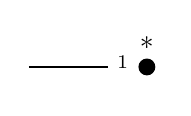
\begin{tikzpicture}
	\draw[thick] (0,0) -- (1,0);
	\node at (1.2,0) {$\A^1$};
	\draw[fill] (1.5,0) circle (0.1cm);
	\node at (1.5,0.3) {$*$};
	\end{tikzpicture}
	\]
$V(I)$, $k[t]$ is a PID.
$I= (f)= ((t-a_1)^{m_1} \cdots (t-a_n)^{m_n})$
$V(f)= \cup (t-a_i)$ finite set of $(t-a_i)$ points
$V((0))= \spec k[t]$
$*= (0)$, its closure is all of $\spec k[t]$
$(0)$ is called the generic point

(3) $\spec \Z$. $\Z$ is a PID so works the same way, so discrete version of the above
	\[
	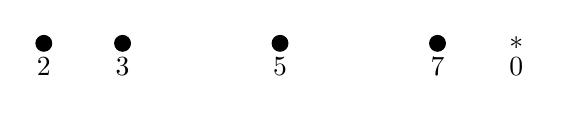
\begin{tikzpicture}
	\foreach \i in {2,3,5,7}
	{
		\draw[fill] (\i,0) circle (0.1cm);
		\node at (\i,-0.3) {\i};
	}
	\node at (8,0) {$*$};
	\node at (8,-0.3) {$0$};
	\end{tikzpicture}
	\]
primes $(p)$ where $p$ prime and $(0)$.

(4) $\spec k[x,y]$ $k$ algebraically closed.
maximal ideals $(x-a,y-b)$, which is $\A^2$
nonmaximal primes $\leftrightarrow$ curves

for each irreducible curve you have an extra point whose closure is that curve.
closure of $(0)$ is whole thing.
\end{ex}



\begin{prop}
Let $k$ be an algebraically closed field and $I,J$ ideals in $k[x_1,\ldots,x_n]$. Suppose $\sqrt{I}= \sqrt{J}$, then $\spec k[x_1,\ldots,x_n]/I$, $\spec k[x_1,\ldots,x_n]/J$ and $\spec k[x_1,\ldots,x_n]/\sqrt{J}$ are all homeomorphic. 
\end{prop}

\pf Primes in $k[x_1,\ldots,x_n]/I$ coorespond to primes in $k[x_1,\ldots,x_n]$ correspond to primes in $k[x_1,\ldots,x_n]$ containing $\sqrt{I}$ correspond to primes in $k[x_1,\ldots,x_n]/ \sqrt{I}$. Obvious bijection between $\spec k[x_1,\ldots,x_n]/I$ and $\spec k[x_1,\ldots,x_n]/\sqrt{I}$.

Let $K$ be an ideal of $k[x_1,\ldots,x_n]/I$ corresponding to an ideal $K' \supseteq I$ of $k[x_1,\ldots,x_n]$. $V(K)$ is primes containing $K$ these correspond to primes containing $K'$ which are the same as primes containing $\sqrt{K}$. $K' \supseteq I$ then $\sqrt{K'} \supseteq \sqrt{I}$, so $\sqrt{K'}$ corresponds to an ideal $L$ in $k[x_1,\ldots,x_n]/ \sqrt{I}$. Thus in the bijection between $\spec k[x_1,\ldots,x_n]/I$ and $\spec k[x_1,\ldots,x_n]/\sqrt{I}$, $V(K)$ goes to $V(L)$. Closed in $\spec k[x_1,\ldots,x_n]/I$ goes closed in $\spec k[x_1,\ldots,x_n]/ \sqrt{I}$. Reverse is similar and easier. \qed \\


$\spec$ does not distinguish between ideals with the same radical. You need to put a sheaf on it. 


\begin{dfn}
Sheaf of rings $\O$ on $\spec A$. For each prime ideal $\fp \subseteq A$, let $A_\fp$ be the localization of $A$ at $\fp$. For an open set $U \subseteq \spec A$, we define $\O(U)$ to be the set of functions $s: U  \to \sqcup_{\fp \in U} A_\fp$ (disjoint union) such that $s(\fp) \in A_\fp$ for each $\fp$ and such that $s$ is locally a quotient of elements of $A$. To be precise, we require that for each $\fp \in U$, there is a neighborhood $V$ of $\fp$ contained in $U$, and elements $a,f \in A$ such that for each  $q \in V$, $f \notin Q$ and $s(q)= a/f$ in $A_q$.  
\end{dfn}


Easy to see its a ring, restriction maps are just restriction of functions. 

Presheaf obvious
extra conditions for sheaf. 
(3) Easy to see restriction of functions 
(4) because of local definition


Let $A= A(X)$ the coordinate ring of an affine variety. $\spec A \supseteq \text{max }\spec A$, where you only look at maximal ideals. $\text{max }\spec A$ with induced topology is homeomorphic to $X$. If $\fm$ is maximal, $(A_\fm)_\fm= k$. 

section $s: U \to \sqcup_{\fm \in U} A_\fm \to k$, composition old fashioned regular function. 


\begin{dfn}
Let $A$ be a ring. The spectrum of $A$ is the pair consisting of the topological space $\spec A$ together with the sheaf of rings $\O$ defined above. For $f \in A$, denote by $D(f)= \spec A \setminus V((f))$ be the primes that do not contain $f$. Open. These $D(f)$ are the basis for a topology on $\spec A$.
\end{dfn}


$V(I)$ closed $\fp \notin V(I)$. 
$\fp \not\supseteq I$ so there is $f \in I$
$f \notin \fp$, $\fp \in D(f)$
$D(f) \cap V(I)= \emptyset$.


\begin{prop}
Let $A$ be a ring and $(\spec A, \O)$ its spectrum. 

\begin{enumerate}[(a)]
\item For any $\fp \in \spec A$, the stalk $\O_\fp$ of the sheaf $\O$ is isomorphic to the local ring $A_\fp$.
\item For any element $f \in A$, the ring $\O(D(f))$ is isomorphic to the localized ring $A_f$
\item In particular, $\Gamma(\spec A, \O) \cong A$. 
\end{enumerate}
\end{prop}


\begin{rem}
(a) Should remind you of the fact that in the old fashioned variety world, you could compute local rings by localization. 

(b) another way to picture $\O(U)$ at least for the D(f)'s

(c) This shows that the pair $(\spec A, \O)$ can now distinguish between $k[x_1,\ldots,x_n]/I$ and $k[x_1,\ldots,x_n]/\sqrt{I}$ when $I \neq \sqrt{I}$. 
\end{rem}


\pf
(a) define a homomorphism $\O_\fp \to A_\fp$. 
$\langle U,s \rangle$, $s \in \O(U)$, $U$ neighborhood of $\fp$. 
$s(\fp) \in A_\fp$. 

$\varphi$ is surjective:
any element of $A_\fp$ has the form $a/f$, $a,f \in A$, $f \notin \fp$.
$D(f)$ will be an open neighborhood of $\fp$.
$\langle D(f), a/f \rangle$. 

injective: 
$U$ neighborhood of $\fp$
$s,t \in \O(U)$ with 
$s(\fp)= t(\fp) \in A_\fp$
shrinking $U$ if necessary, we may assume
$s= a/f, t= b/g$ on $U$
where $a,b,f,g \in A$, $f,g \notin \fp$

$a/f= b/g$ in $A_\fp$
there exists $h \notin \fp$
$h(ga-fb)=0$ in $A$

Therefore, $a/f= b/g$ in every local ring $A_q$
such that $f,g,h \notin q$.
The set of such $q$ is 
$D(f) \cap D(g) \cap D(h)$, which contains $\fp$

This is a smaller open set on which $s=t$
so they are equal in $\O_\fp$.

(b)(c)
(c) is (b) with $f=1$ as $D(1)= \spec A$. 
So suffices to prove (b).

$\psi: A_f \to \O(D(f))$
$a/f^n \to s$ which assigns $s(\fp)= a/f^n \in A_\fp$. 
check that it is a homomorphism

injective: $\psi(a/f^n)= \psi(b/f^M)$ then
for every $\fp \in D(f)$, $a/f^n$ and $b/f^m$
have same image in $A_\fp$
$h \notin \fp$, $h(f^ma - f^nb)= 0$ in $A$.

Let $I$ be the annihilator of $f^ma - f^nb$. Then $h \in I$ and $h \notin \fp$ so $I \not\subseteq \fp$. This holds for every $\fp \in D(f)$. 





























